\chapter{Внедрение БШС на нефтегазовых месторождениях}\label{ch:ch1}


Цифровая трансформация является первостепенной задачей для развития нефтегазового комплекса. Переход производства к новой модели управления <<Индустрия 4.0>> позволит бизнесу сохранить лидирующие позиции и не утратить производственного потенциала  \cite{Eremin2020, Dmitrievskiy2020}. Неотъемлемой частью такой трансфомарции является внедрение беспроводных технологий \cite{Eremin2020, Dmitrievskiy2020, Eremin2019, Hiriyannaiah2020, Munirathinam2020, CarmenLucas-Estan2018}. 


Современные беспроводные широкополосные сети связи (БШС), обладая рядом преимуществ, нашли свое широкое применение в задачах мониторинга и управления различных   производственных или гражданских объектов, технологических установок, движущихся транспортных средств и т.п. К ряду таких преимуществ можно отнести возможность получения информации с любой точки контролируемой территории, быстрый ввод в эксплуатацию, сокращение капитальных затрат на создание и эксплуатацию сети, высокая гибкость, мобильность и масштабируемость. 


Нефтегазовые объекты часто расположены в труднодоступной местности на обширной территории в несколько киллометров. Данный фактор является ключевым преимуществом беспроводных технологий для развертывания по сравнению с кабельными коммуникациями.

Беспроводная связь в автоматизации промышленного производства способствует осуществлению производственных процессов более экономически эффективно, гибко и надежно, а также позволяет реализовывать новые концепции автоматизации \cite{Gost62657}. Для управления большими объемами на месторождениях применение применение беспроводных каналов связи в режиме 60/24/7, позволяюшая операторам принимать обоснованные управленческие решения, своевременно диагностировать и устранять неисправности, а также оптимизировать работу АСУ ТП в целом \cite{Dmitrievsky2021}.

Не маловажную роль на месторождениях играет безопасность. Технологические объекты на нефтяных или газовых месторождениях, оснащенных широкополосным подключением, позволяют соответствовать современным концепциям и требованиям в сфере безопасности персонала и безопасности имущества, включая охрану с использованием беспроводных камер видеонаблюдения. Для предоставления доступа к объекту могут использоваться дополнительные возможности, такие как считывание номерных знаков и распознавание лиц. А благодаря использованию тепловых камер можно контролировать риски отключения и перегрузки даже с помощью периодических снимков оборудования на промысле. 

Внедрение БШС особенно хорошо подходят для систем видеонаблюдения, поскольку позволяют расположить камеры там, где они нужны, а не там, где удобно для подключения к проводной сети.

В данном исследовании в рамках цифровой трансформации <<Индустрия 4.0>> представлены модели и методы оптимизации при проектировании беспроводных сетей на месторождениях  (Рисунок \cref{fig:industry4}).

\begin{figure}[h!]
  \centering
   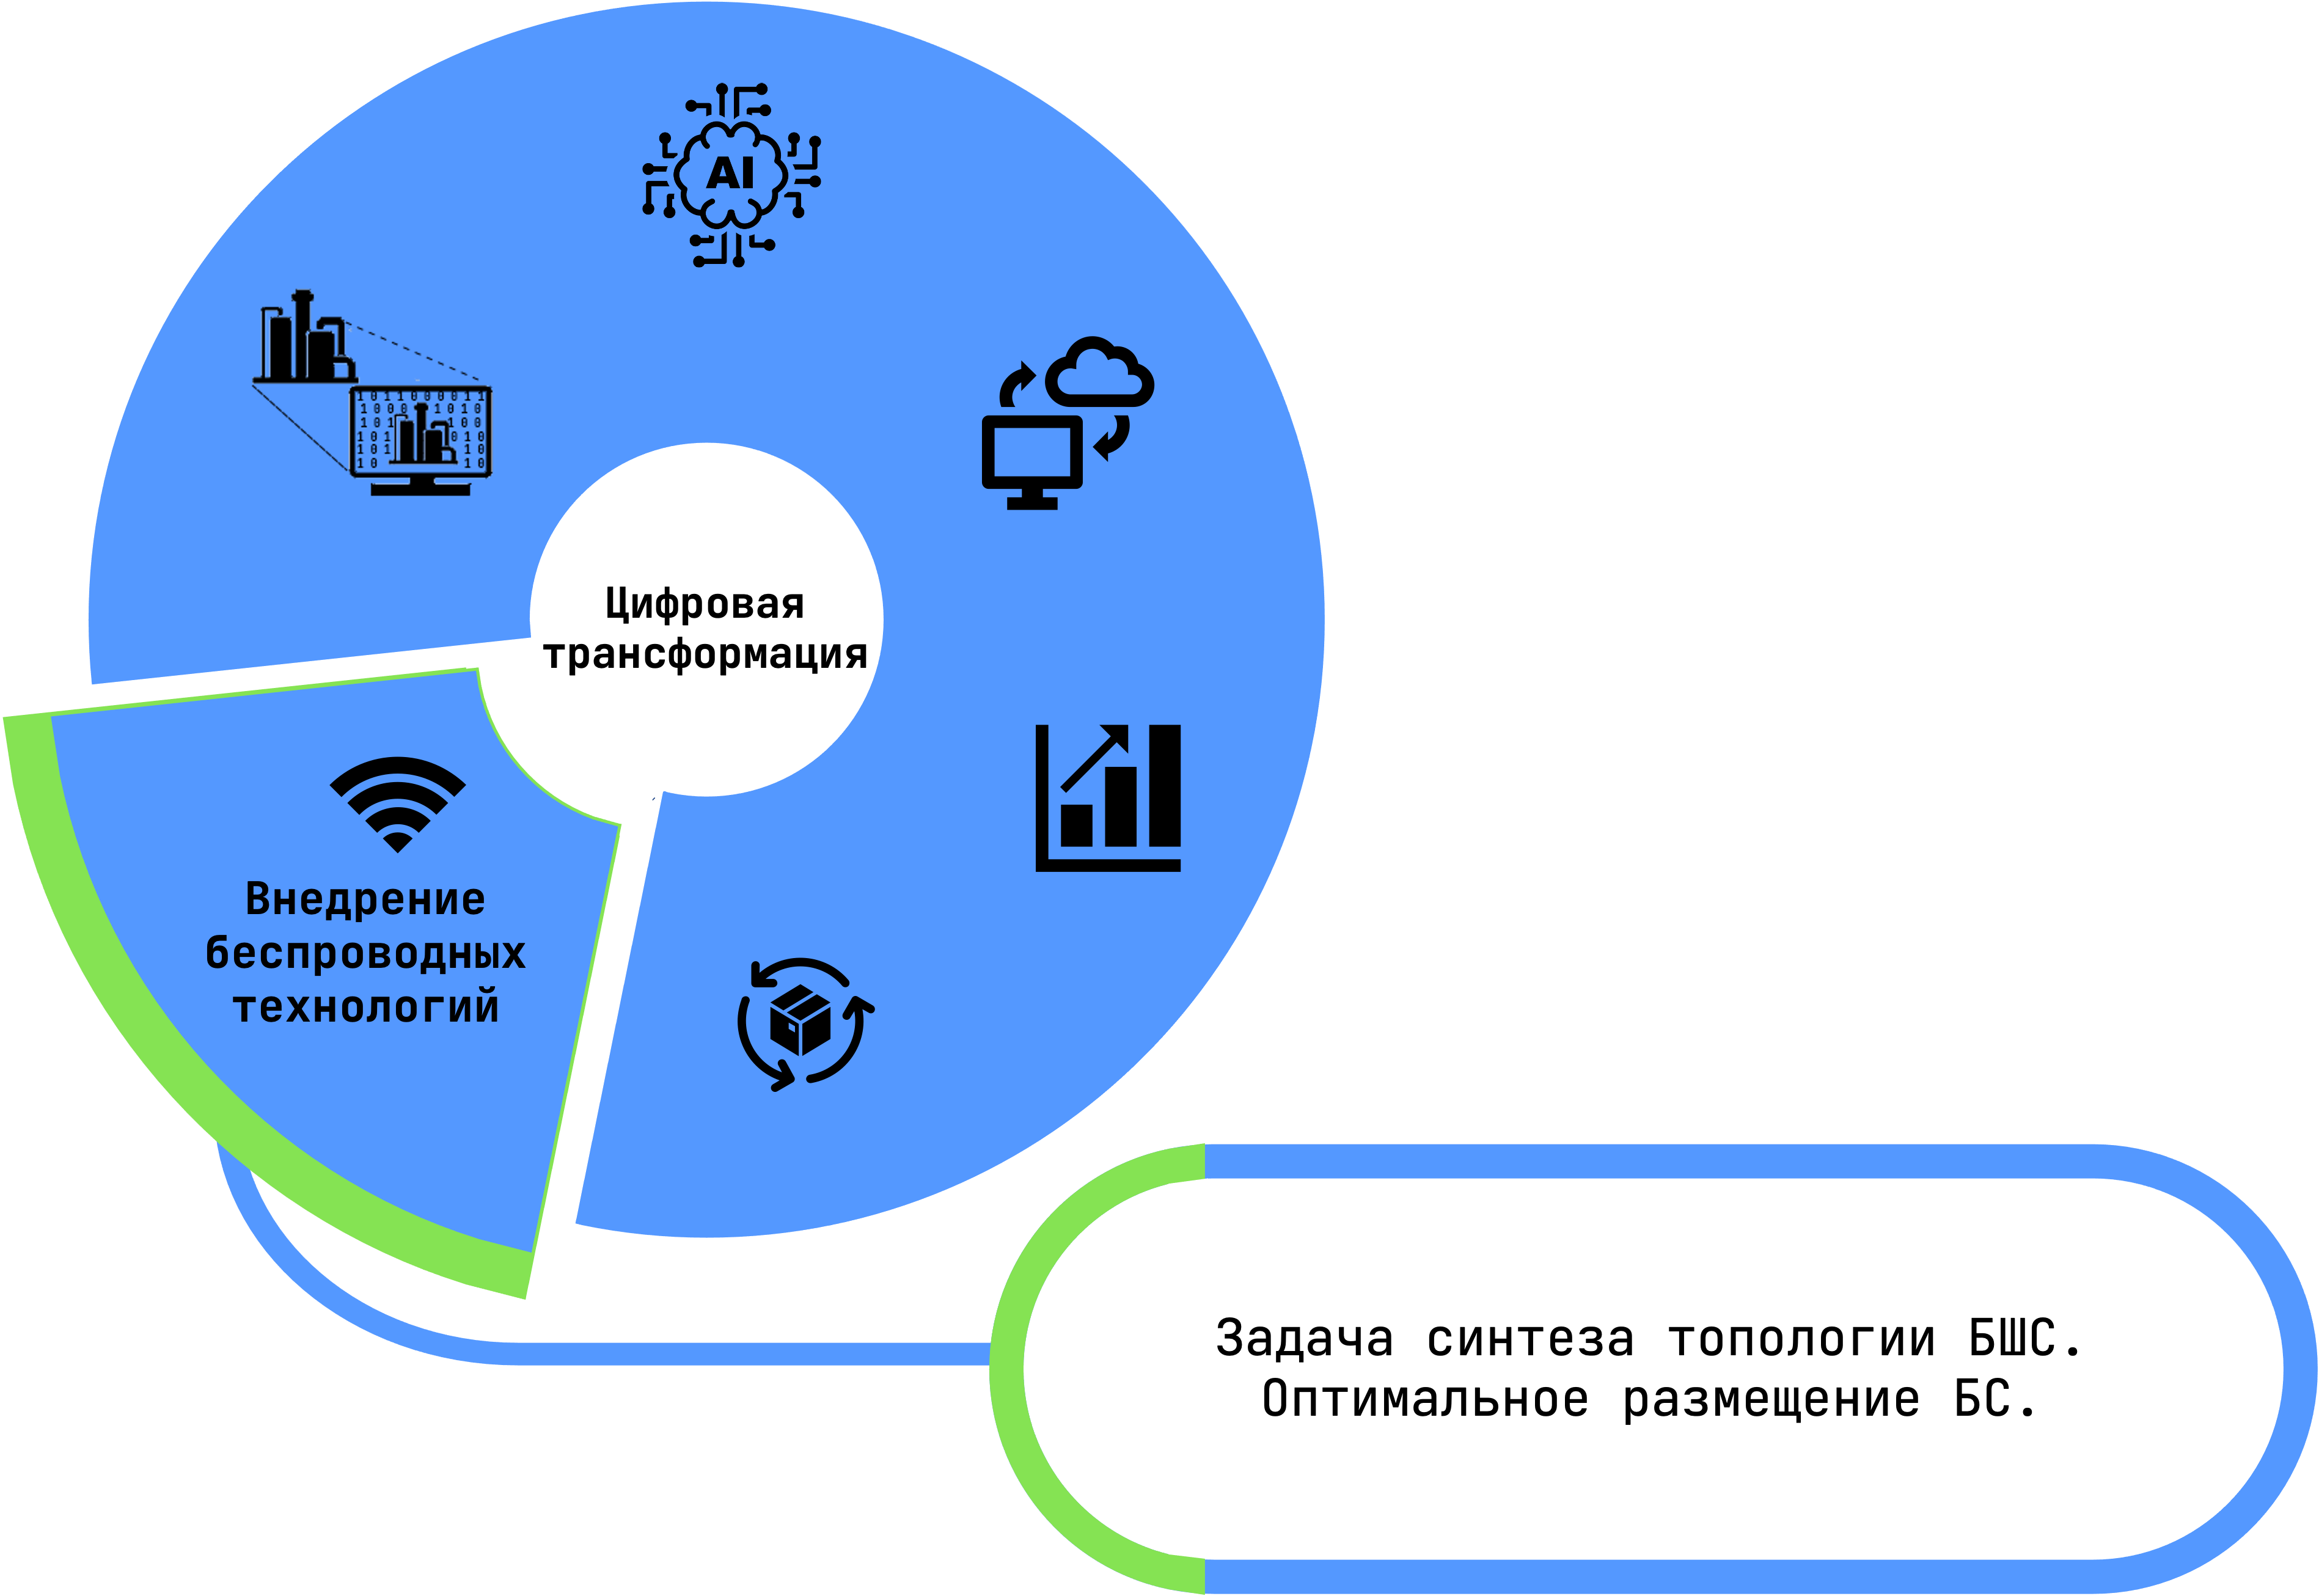
\includegraphics[width=1\textwidth]{industry4.png}
\caption{Задача синтеза топологии при проектировании БШС в рамках цифровой трансформации "Индустрия 4.0".}
\label{fig:industry4}
\end{figure}



\section{Этапы проектирования БШС}

Для обеспечения высокого качества беспроводной связи необходимо проводить грамотное проектирование БШС. Существуют различные подходы к проектированию беспроводных сетей. Для одних задачей является максимальная зона покрытия, для других -- достижения максимальной производительности передачи данных, для третьих -- нахождения баланса между зоной охвата и производительностью \cite{Proletarsky}. В диссертации будут предложены модели и методы оптимального размещения базовых станций (БС) БШС, целью которых является максимальная зона охвата.  Процесс проектирования современной БШС, как правило, для такого подхода имеет следующие основные этапы (Рисунок \cref{fig:part1_design_stages}):

\begin{figure}[h!]
  \centering
   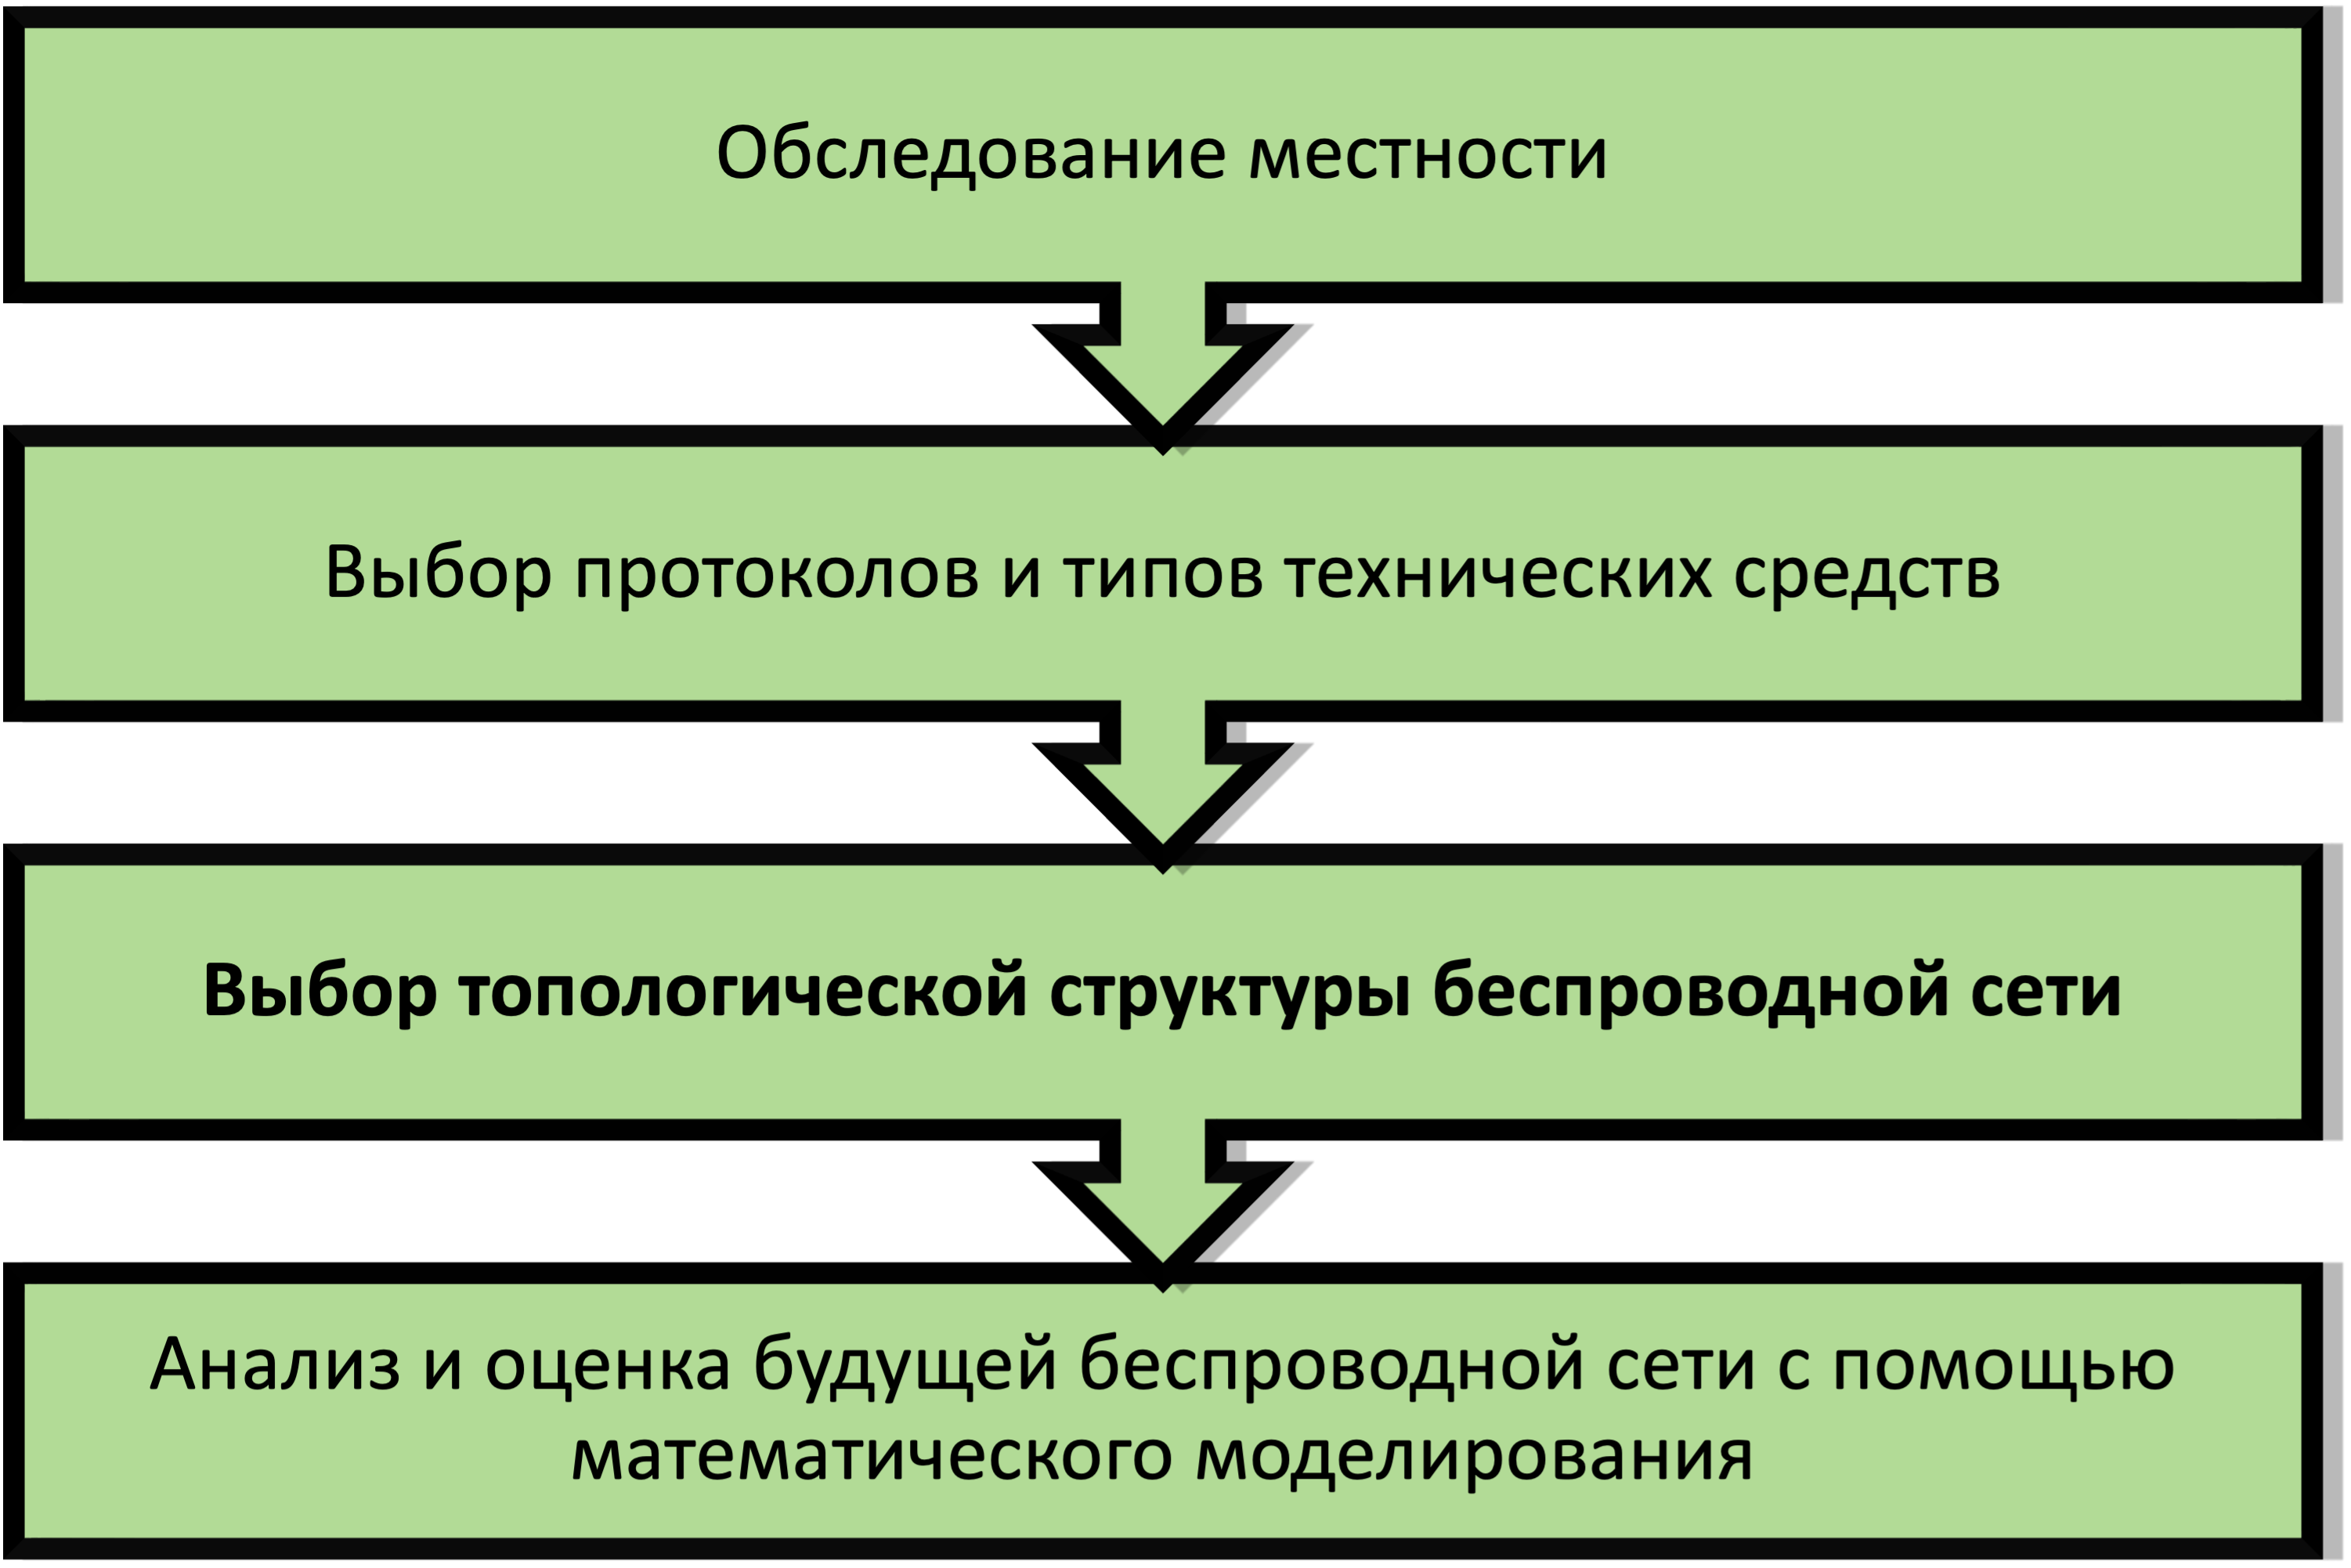
\includegraphics[width=0.8\textwidth]{design_stages.png}
\caption{Этапы проектирования БШС.}
\label{fig:part1_design_stages}
\end{figure}

Любое проектирование БШС всегда начинается с первоначального обследования местности. В данный этап входят задачи радиобследования и радиопланирования. оценки реальных размеров области контроля, наличие стационарных инженерно-технических сооружений, мешающих передачи сигнала, такими как металлические конструкции, перекрытия, стены и т.д. При развертывании БШС в открытой местности также немаловажную роль играет наличие перепада высот. В ходе выполнения комплекса работ на местности, определяются возможные точки размещения оборудования \cite{Dunaitsev2017}. На основе результатов данного этапа проводится выбор типов моделей оборудования для дальнейшего их размещения и организации сети.

Производительность и дальность действия беспроводных сетей не безграничны. При их проектировании стоит учитывать множество параметров: частота, скорость, мощность излучения \cite{Proletarsky}. На этапе выбора оборудования необходимо определиться с протоколом будущей БШС и  подготовить необходимый комплекс технических средств для развертывания будущей сети. БС является основополагающем устройством будущей сети, которая отвечает за покрытие заданной области. Покрытие в свою очередь зависит от мощности передатчика устройства, усиления антенн, чувствительности приемного устройства.


После определения множества возможных точек размещения БС на этапе обследования местности и выборе возможных типов и моделей оборудований можно переходить непосредственно к размещению БС и определению топологической структуры сети. Этап выбора топологической структуры будущей сети является ключевой проблемой данной диссертации. В рамках данной проблемы будут предложены модели и методы оптимального размещения БС для организации БШС.

После решения задачи синтеза топологии, для полученного размещения решаются задачи оценки характеристик производительности БШС. Для расчета оценок широко применяется аппарат теории массового обслуживания (ТМО). Примерами таких задач являются расчет надежности всех элементов сети \cite{Wankpo2020, Krishnamoorthy2021, Kozyrev2019}, оценка характеристик качества канала, вероятности потери пакетов, пропускной способности, времени доставки сообщений в сети \cite{Gorbunova2020, Larionov2019, Vishnevsky2016_Methods_of_performance, Vishnevsky2016_Review_of_methodology, Wang2017, Sandmann2012, Baumann2017}, оценка межконцевой задержки сети \cite{Wang2017, Sandmann2012}. В работе \cite{Eremenko2013} рассматривают стохастическую модель марковской цепи для оценки качества передачи данных автоматизированных систем управления технологическим процессом (АСУ ТП) в условиях помех и прерываний. Одним из современных направлений в исследовании характеристик производительности БШС является использование ТМО в совокупности с методами машинного обучения (МО) \cite{Lovas2021, SatyaHermanto2018}.

Описанная процедура проектирования БШС является общей для большинства внедрения беспроводных коммуникационных сетей. В зависимости от конкретных целей, которые преследуют проектировщики, план работ может требовать содержание конкретных этапов и подзадач проектирования. В общем же случае проектирование БШС будет происходить согласно данной последовательности этапов. В изложенной концепции важным является представление места результатов исследования данной диссертации в глобальной задаче комплексного проектирования.


\section{\fixme{Анализ современных беспроводных широкополосных технологий передачи данных}}

Существуют множество различных протоколов БШС, используемых на месторождении. Любая сеть имеет свои преимущества для конкретной задачи. Исходя из специфики таких задач, можно выделить два больших класса. Первый класс -- это сети, узлами которого являются измерительные устройства (сенсоры) АСУ ТП. Такие сети называются  ячеистые сенсорные сети. Для таких сетей характерны низкоскоростной трафик, малое энергопотребление, высокие требования к надежности передачи, а также надежности, непосредственно,  оборудования. Вторым классом сетей являются БШС, для которых  характерны высокая скорость передачи, большая дальность передачи сигнала от несколько десятков метров до несколько сотен метров. Примерами таких сетей являются сети второго уровня, объединяющие кластеры сенсорных сетей для передачи данных в центр управления. Также примером является БШС сбора мультимедийного трафика с беспроводных камер видеонаблюдения. 

\subsection{Ячеистые сенсорные сети c низкоскоростным трафиком}
Нижний уровень АСУ ТП, включающий измерительные приборы технологических параметров, исполнительные механизмы, коммутируемые с устройствами сопряжения, объединяются в беспроводную сенсорную сеть для эффективного мониторинга, контроля и управления технологическим объектом \cite{Florencio2020}.


Ячеистая сеть (Mesh) является одной эффективных технологий, позволяющая работать в неблагоприятных климатических условиях \cite{Sidney2015} \fixme{Добавить обзор}. Ячеистые сети имеют повышенную надежность благодаря тому, что каждое устройство является узлом такой сети, через который помимо сигнал с самого устройства передается сигнал смежных узлов сети.
Сеть на основе ячеистой топологии надежна, энергоэффективна. Высокая надежность обеспечивается наличием резервных маршрутов передачи данных. При прекращении функционирования одного из устройств (датчиков), передача сигнала будет происходить в обход устройства, по резервному пути. Ключевым недостатком MESH сетей является -- низкая скорость передачи данных. К ключевым преимуществом сенсорных сетей можно также отнести автономность питания, позволяющее установку узлов (устройств) сети на удалении от проводных сетей и общего питания. 


Благодаря невысокому энергопотреблению устройств ячеистые сенсорные сети могут работать продолжительное время от одного элемента питания. Это осуществляется за счет управления временем опроса данных в диапазоне от одной секунды до одного часа. Такой подход позволяет  экономить заряд батареи устройства и увеличивает продолжительность жизни устройства.

Широкое распространение в промышленности получили протоколы сенсорных сетей: ISA100.11a, ZigBee, WirelessHART и набирающий свою популярность стандарт LoRaWAN. Производители сенсорных сетей Emerson, Honeywell, Yokagawa, Simens и др. обеспечивают высокую надежность узлов таких сетей, так как работа оборудования осуществляется в условиях пыли, влаги, вибраций и высоких температур.

\subsubsection{ISA 100.11a}
Данный протокол является одним из распространенных протоколов передачи сигнала на промысле. Так компания Honeywell Process Solutions приняла решение разрабатывает оборудование, совместимое с ISA 100 Wireless \cite{Sidney2015}.
Топология, используемая в ISA 100.11a, основана на соединении типа "точка -- точка". Такая сеть представляет собой централизованную систему, где каждое полевое устройство связано непосредственно с главным устройством (шлюзом). 

Протокол ISA 100.11a определяют следующие методы: расширенный спектр со скачкообразной перестройкой частоты (FHSS), множественный доступ с временным разделением каналов (TDMA) и множественный доступ с контролем несущей (CSMA).

Как и любая MESH сеть, данная технология энергоэффективной, т.е. с меньшим энергопотреблением для мощности передачи сигнала. Данный фактор вносит существенную проблему, каждое устройство должно быть в непосредственной близости от шлюза и иметь прямую видимость для передачи данных. Для решения этой проблемы, в стандарт была добавлена поддержка Mesh. Потеря связи и плохой сигнал сказываются не только на целостности и своевременности получаемой информации, но и на жизненном цикле батареи питания \cite{Tagirov2013}.

\subsubsection{ZigBee}
Технология Zigbee основана на протоколе IEEE 802.15.4 LR PAN (Low Rate Personal Area Network) для низкоскоростных сетей с малым энергопотреблением. Этот стандарт описывает физический и канальный уровни со скоростью обмена данными до 250 Кбит/с и вариантами топологии "звезда","точка-точка" и Мesh. Частотный диапазон сети для России 2400 - 2483 МГц (16 каналов). Дальность связь -- 200 м. Стандарт поддерживает до 255 одновременно подключенных устройств. Ключевым преимуществом ZigBee является низкое энергопотребление. Исторически технологии ZigBee развивалась не в направлении повышения скорости передачи данных, а по пути улучшения алгоритмов сетевого взаимодействия для обеспечения длительного время работы без замены электропитания.  В сетях ZigBee различают два типа устройств -- полнофункциональные устройства FFD (Full-Function Device) и устройства с сокращенным набором функций  RFD (Reduced-function Device). Устройство FFD выступает в роли координатора, то есть организующего сеть и ретранслирующего сообщения. Устройства RFD не могут обмениваться данными друг с другом, а только через координатор FFD.

Сеть ZigBee строится на базе трех основных устройств: координатор, оконечное
устройство и маршрутизатор. Координатор выполняет основную роль в сети: формирует,
запускает сеть, участвует в построении сети, управляет ею, выполняет функции
маршрутизатора и доверительного центра (trust-центра) – устанавливает настройки
безопасности, задает настройки в процессе присоединения устройств к сети, управляет
ключами безопасности [3]. 

\subsubsection{WirelessHART}


Протокол WirelessHART разработан для мониторинга на базе проводного протокола HART с выходным сигналом 4 -- 20 мА. Верхний стек WirelessHART соответствует верхним уровням HART и Modbus. Первой компанией, которая предоставила оборудование, поддерживающее WirelessHART была Emerson. Технология также, как и ZigBee, соответствует стандарту IEEE 802.15.4, работающая в частотах не лицензируемого диапазона ISM (промышленность, наука и медицина) —- 2400–2483,5 МГц.

Координация коммуникации в сети c одноуровневым кодированием осуществляется посредством метода множественного доступа с временным разделением каналов (Time Division Multiple Access – TDMA), который синхронизирует радиостанции с периодом 10 мс \cite{Chupaev2018}. Шлюз системы WirelessHART поддерживает до 250 полевых устройств. 

В WiressHART используется широкополосная модуляция методом прямой последовательности DSSS. Для предотвращения интерференции с сетями, работающими на этой же частоте, предусмотрена технология скачкообразной смены несущей частоты (FHSS) \cite{Tagirov2013}

\subsubsection{LoRaWAN}
LoRaWAN -- современный стандарт интернета вещей (IoT) с большим потенциалом. Применяется для передачи низкоскоростного трафика. Данная технология только начала осваивать промышленный сектор. К преимуществам LoRaWAN относят очень высокую чувствительность приемника до -148 дБм, большая дальность связи 10-15 км и низкое энергопотребление у конечных устройств. По сравнению с другими энергоэффективными сетями LoRaWan имеет колоссальную дальность коммуникационной связи. Демодулятор LoRa может работать при входном сигнале, ниже уровня собственных шумов, вплоть до -20 дБ \cite{Yang2020}. 

Низкое энергопотребление осуществляется за счет передачу небольших пакетов данных. Это в свою очередь приводит к относительно низкой пропускной способности. Скорость передачи в зависимости от используемой технологии передачи данных на физическом уровне варьируется от нескольких сотен бит/с до нескольких десятков Кбит/с.



\fixme{Почитать про LoRaWAN. Может быть подойдет под задачу на плоскости.}


\subsection{Сети дальнего радиуса действия с высокоскоростным трафиком}

Ячеистые сенсорные сети давно и прочно вошли как неотъемлемая часть АСУ ТП на производстве. Тем не менее они имеют один существенный недостаток -- малый радиус действия связи. Для решения такой проблемы, кластеры ячеистых сетей объединяет между собой в иерархическую структуру, в которой шлюзы объединяются в сети, на базе протоколов дальнего радиуса действия: Wi-Fi, WiMAX \cite{Savazzi2013}. Такие технологии организуют второй уровень, после уровня сбора и обработки информации с полевых устройств, для передачи данных в центр управления. Еще одним современным направлением является внедрений сетей телекоммуникаций для обеспечения связи для мобильных устройств обходчиков и сбора данный с беспроводных камер видеонаблюдения \cite{Sidney2015}.







\subsubsection{WiMAX}
Технология WiMAX основана на стандарте IEEE 802.16. Разработанный стандарт беспроводной широкополосного доступа рассчитан на внедрение в городских распределенных региональных беспроводных сетях в диапазонах до 66 ГГц. Стандарт предусматривает 5 режимов работ. Режим магистральной передачи WirelessMAN-SC работает в диапазоне 10-66 ГГц со скоростями до 120 Мбит/с и шириной канала порядка 25 МГц. Применяемые топологии -- "точка-точка" и "точка - много точек" \cite{Vishnevsky2009}. Остальные режимы WirelessMAN-SCa, WirelessMAN-OFDM, WirelessMAN-OFDMA и  WirelessHUMAN работают на частотах 2-11 Ггц. Режим WirelessMAN-OFDM поддерживает архитектуру Mesh. Дальность связи для WiMAX технологии достигает 20 км для прямой видимости и хорошего состояния радиоканала.

На сегодня технология применяется в качестве организации резервированного канала связи для сбора данных с кустовых площадок с блока местной автоматики в диспетчерский пункт и мультимедийного трафика с систем видеонаблюдения. 

Технология WiMAX успела получить свою популярность на месторождениях и занять свою нишу в организации телекоммуникационной связи. Исторически WiMAX всегда рассматривался как альтернатива сотовым сетям связи. С резким скачком популярности LTE и появлением сетей пятого поколение WiMAX давно уже является не конкурентным стандартом на рынке.

\subsubsection{Wi-Fi}

Семейство протоколов IEEE 802.11 или Wi-Fi является одним из популярных протоколов среди беспроводных сетей широкополосного доступа. Широкое применение Wi-Fi не могло не отразиться и на нефтегазовом секторе \fixme{ДОБАВИТЬ ОБЗОР wifi oil gas}. 

Стандарт определяет два типа топологий. Первая топология в стандарте называется независимой (Independent Basic Service Set, IBSS) на основе "точка-- точка". Такую сеть также называют Ad-Hoc сетью. Передача в сети производится на основе децентрализованного алгоритма доступа. Хоть и не существует главной базовой станции, в сети Ad-Hoc в каждый момент времени любой узел может взять ведущую роль базовой станции. Следующий тип -- централизованная топология. Такой тип сети называют Infrastracture  Basic Service Set или просто BSS \cite{Olifer2020}. Узлы сети могут обмениваться только с базовой станцией, обеспечивающее взаимодействие между всеми конечным узлами сети. 
 
Стек протоколов стандарта IEEE 802.11 соответствует общей структуре 802 (Рисунок \cref{fig:part1_wifi_osi_stack}). Физический уровень практически соответствует физическому уровню в модели OSI. Канальный уровень во всех протоколах 802.х разбит на два или более подуровня.  Подуровень управления доступа к среде обеспечивает адресацию и механизмы управления доступом к каналам. Подуровень MAC выступает в качестве интерфейса между физическим уровнем и подуровнем управления логическим соединением (LLC). Задача LLC состоит в том, чтобы сделать различия стандартов 802.11x невидимыми для сетевого уровня \cite{Tanenbaum2022}. На уровне MAC протокола 802.11 определяются два типа доступа к среде передачи данных: функция распределенной координации (Distributed Coordination Function, DCF) и функция централизованной координации (Point Coordination function, PCF), работающий только в режиме IBSS \cite{802.11WG-WirelessLANWorkingGroup2020}.


\begin{figure}[h!]
  \centering
   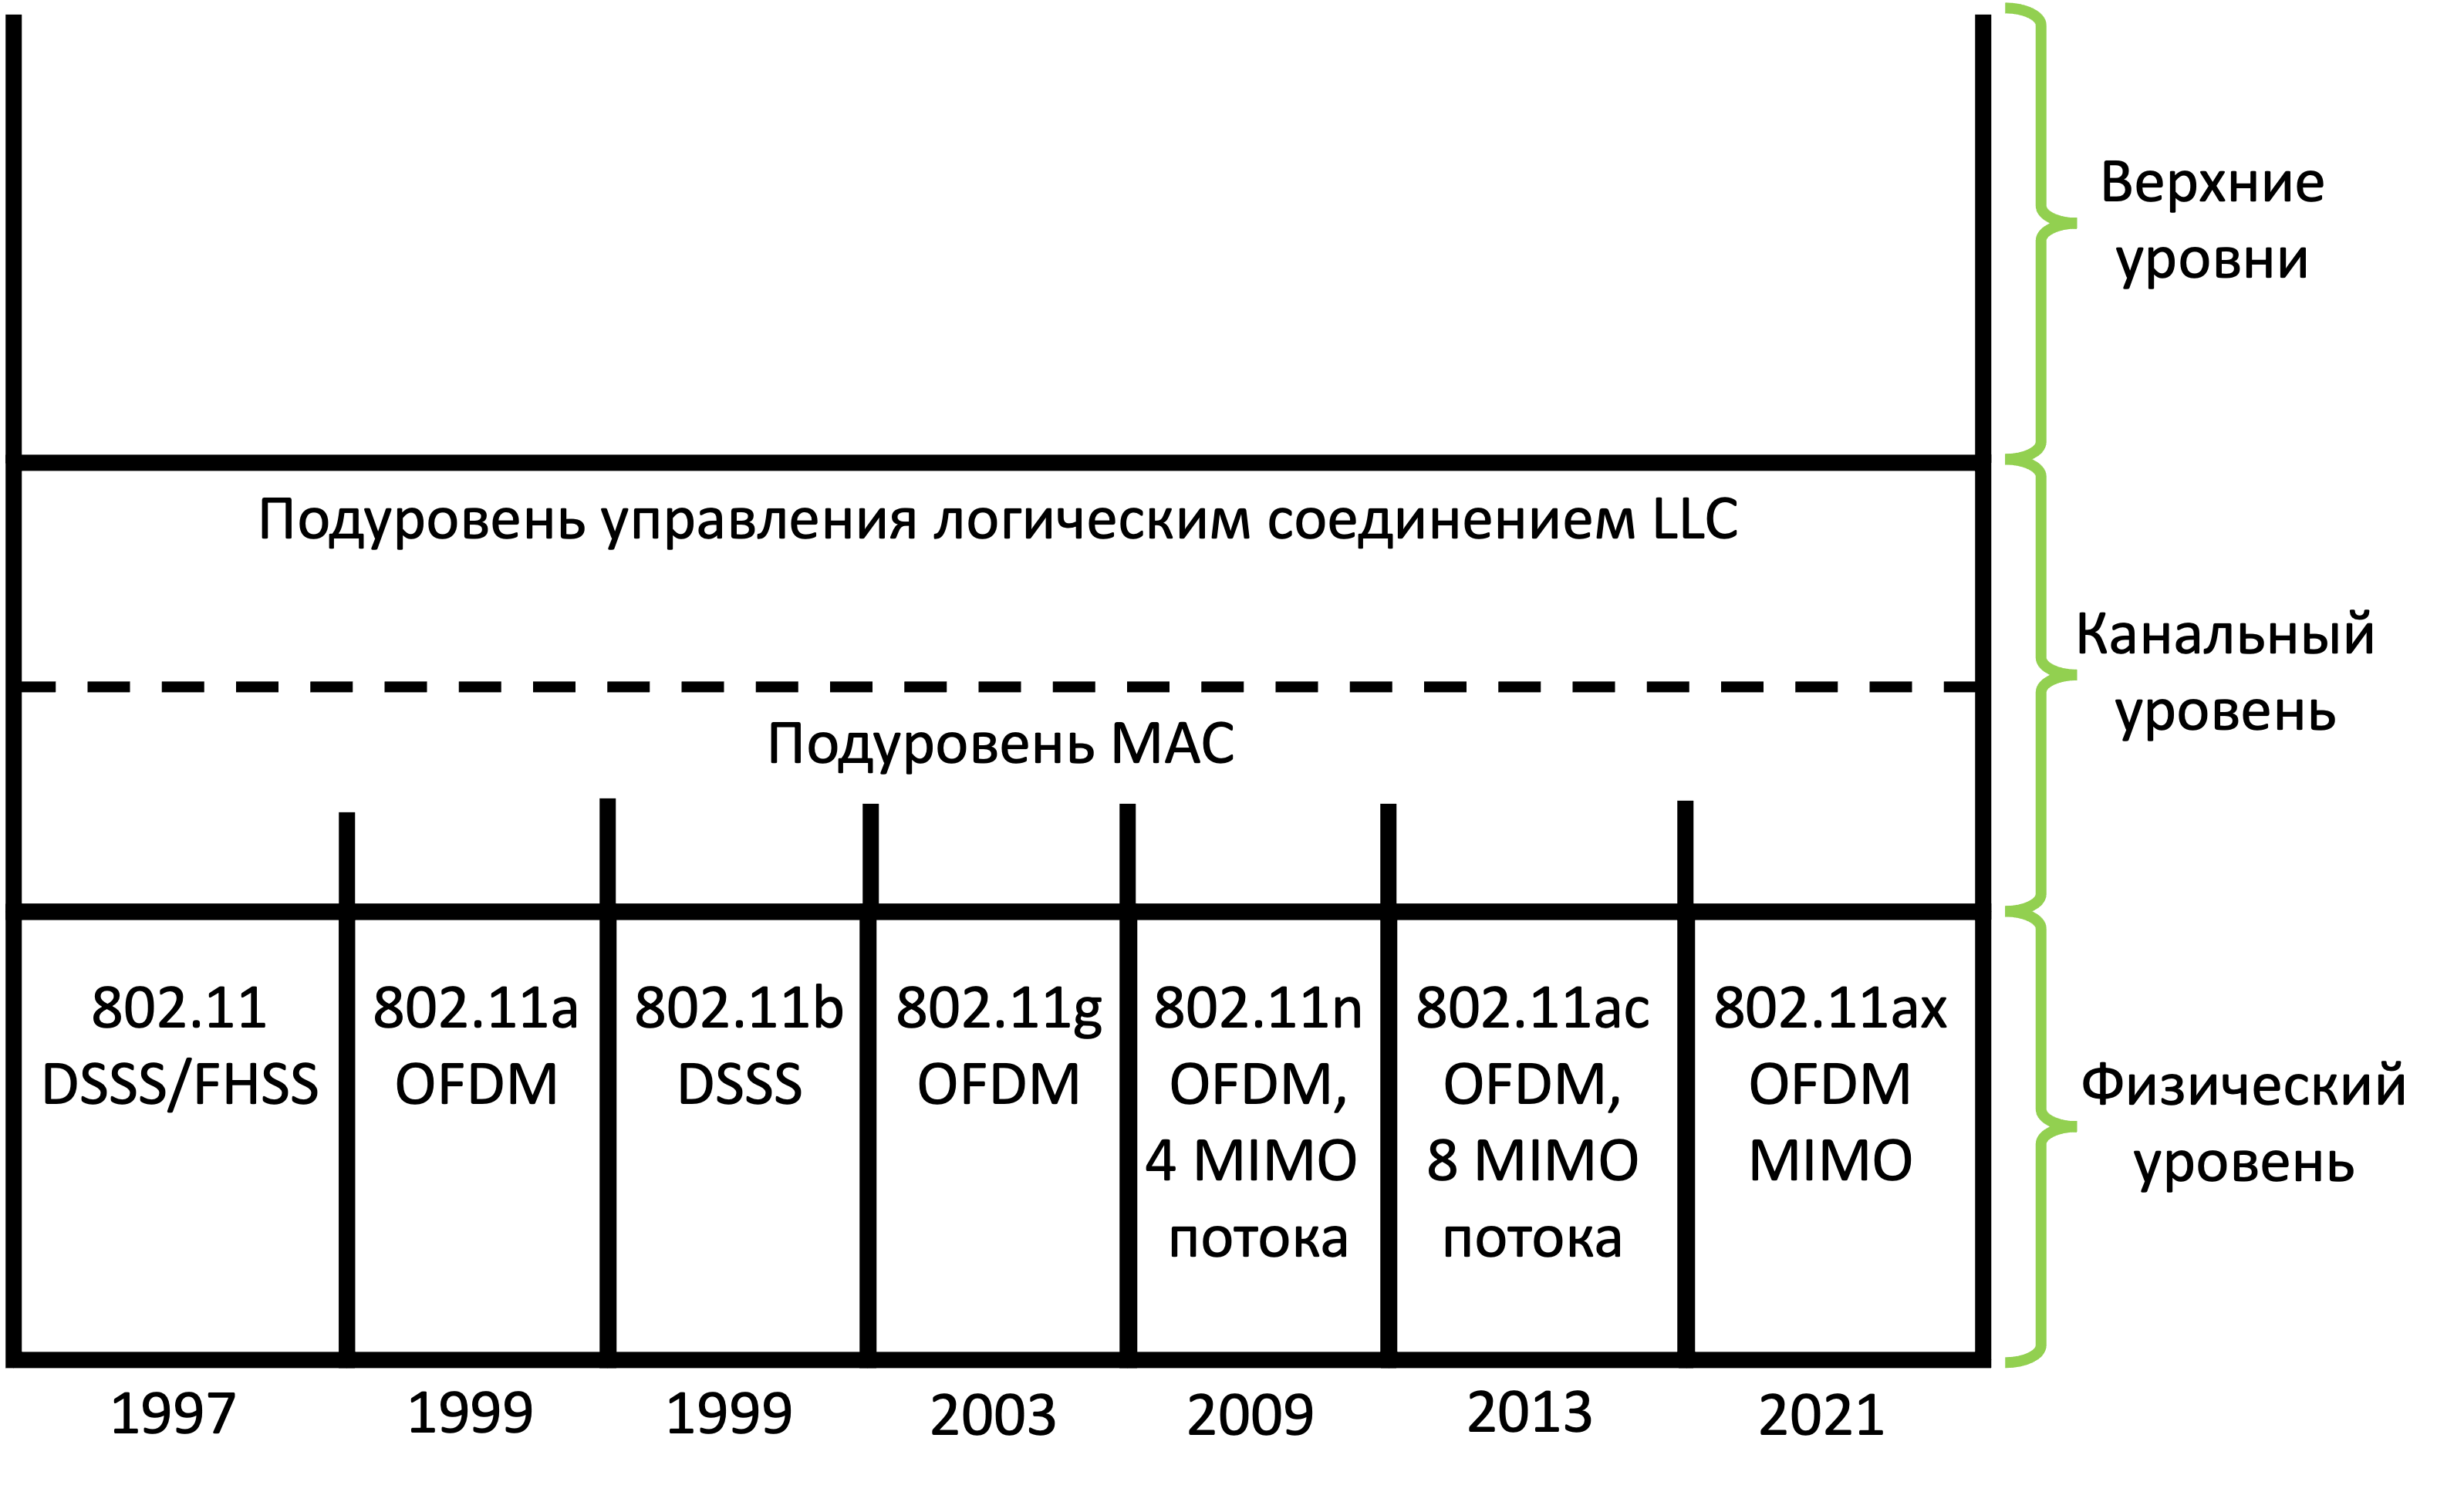
\includegraphics[width=0.8\textwidth]{wifi_osi_stack.png}
\caption{Часть стека протоколов 802.11}
\label{fig:part1_wifi_osi_stack}
\end{figure}

\paragraph{Развитие стандарта.}
Первый стандарт в 1997 году поддерживал скорость передачи до 1,2 Мбит/c с рабочем диапазоном частот 2,4 ГГц. Уже в 1999 году стандарт 802.1b скорость передачи достигала 11 Мбит/с. В тот же 1999 год одновременно вышел 802.11a, поддерживающий способ модуляции OFDM -- мультиплексирование с ортогональным частотным разделением каналов. Данный метод модуляции пришел на смену методов прямой последовательности для расширения спектра (direct sequence spread spectrum, DSSS) и псевдослучайная перестройка рабочей частоты (frequency-hopping spread spectrum, FHSS). Протокол работает в диапазоне частот 5ГГц. Данное введение позволило увеличить скорость до 54 Мбит/с. В 2003 году появился 802.11g, в котором OFDM стал совместим с 802.11b DSSS.  В 2009 году, в рамках стандарта 802.11n была завершена работа над методами передачи данных SU-MIMO (Single User -- Multiple Input Multiple Output), которые одновременно используют несколько антенн на приемнике и передатчике, что дает очередной выигрыш в скорости. Благодаря четырем антеннам и более широким каналам стандарт 802.11 теперь определяет скорости до 600 Мбит/с \cite{Tanenbaum2022, Coleman2018}. В 2013 году появился стандарт 802.11ac с максимальной теоретической скоростью беспроводного соединения 3,47 Гбит/с. В данном стандарте представлена технология одновременная передача по нескольким антеннам сразу четырем клиентам MU-MIMO (Multi User –- Multiple Input Multiple Output). В 2021 была представлена сеть шестого поколения Wi-Fi 6, стандарт получил название IEEE 802.11ax. Скорость передачи достигает 9608 Мбит/с. Стандарт работает на частотах 2,4 ГГц и 5 ГГц. Реализована новый тип модуляции -- 1024-QAM. Теперь MU-MIMO работает для одновременной передачи до восьми клиентам.  Кроме того, Wi-Fi 6 обеспечивает эффективную работу в сетях IoT, существенно повышая эффективность работы с малыми объемами данных и эффективно используя батарею маломощных измерительных устройств за счет сокращения обмена служебной информацией.

\paragraph{Беспроводной широкополосный доступ вдоль протяженных автомобильных дорог.}
Обеспечение безопасности на автодорогах, в том числе на промысле, является  актуальной задачей на сегодняшний день. Одним из методов ее решений является создание современной инфраструктуры передачи мультимедийной информации вдоль протяженных автомагистралей \cite{Vish2015}. Для реализации такой сети разработан стандарт IEEE 802.11p/WAVE. Протокол разработан для обмена данными между высокоскоростными транспортными средствами, а также между транспортными средствами и придорожной инфраструктурой. Такие сети называются V2X (Vehicle-to-everything). 802.11p работает в диапазоне 5,85–5,925 ГГц для движущихся объектов на скорости до 200 км/ч мимо неподвижных базовых станций на расстоянии до 1 км. Протокол IEEE 802.11p входит в состав стандарта Wireless Access in Vehicular Environ (WAVE) и является своего рода интерфейсом для связи с IEEE 1609. В совокупности два этих стандарта определяют интерфейс и набор дополнительных функций для обеспечения связи между движущимися объектами \cite{IEEE802.11p}.

\paragraph{Ячеистая топология стандарта 802.11.} Стандарт поддерживает MESH топологию. Все нововведения относятся к МАС уровню и рассматриваются вопросы маршрутизации пакетов в рамках mesh-сети. Фактически в стандарте рассматриваются сетевой и транспортный уровень модели OSI. Пакет уровня MAC содержит дополнительный MESH - заголовок в отличие от стандартных заголовка пакетов 802.11. В заголовке указывается время жизни пакеты при пересылке через несколько узлов сети \cite{Vishnevsky2009}. Такой подход помогает решить проблему наличия циклов при выборе пути передачи. Протоколы маршрутизации делят на два класса: проактивный -- каждый узел строит свою таблицу маршрутизации и делится информацией об изменении топологии сети со своими соседями и реактивный --  таблицы маршрутизации не строятся, маршрут составляется по мере необходимости. Стандарт 802.11s определяет гибридный протокол маршрутизации по умолчанию -- HWMP (Hybrid Wireless Mesh Protocol). Также стандарт позволяет разработчикам оборудования использовать альтернативные методы маршрутизации. Режим энергосбережения в 802.11s является опциональным \cite{802.11WG-WirelessLANWorkingGroup2020}. Точки доступа MESH-сети (MESH Access Point, MAP) всегда активны, так как в любой момент времени могут обратиться устройства, не поддерживающие непосредственно 802.11s. Необходимость возникает в случае IoT, когда всегда устройства имеют автономное питание (измерительные устройства, датчики) \cite{Vishnevsky2009}.




\fixme{Смартфоны от Honeywell}

\fixme{Рассказать про mesh 802.11s}

% Организация сети для передачи мультимедийного высокоскоростного трафика с камер видеонаблюдения, а также сбор данных с мобильных устройств обслуживающего персонала \cite{Sidney2015} \fixme{Добавить обзор}.



\fixme{БС организуются в сети WiMax и Wi-Fi}

\fixme{Для обеспечения связи между станциями буду использовать Wi-Fi }

При внедрении беспроводных технологий необходимо учитывать специфику выполняемых задач будущей сети. Для каждого конкретной цели существуют свои требования к скорости передачи данных, дальности связи, потребляемой мощности, помехозащищённости, надежности и т.д. Чтобы учесть специфику данных задач разработано множество беспроводных решений, охватывающее дальность связи от несколько сантиметров до десятков километров и скоростей передачи от единиц Кбит/с до сотен Мбит/с.

\subsection{Выбор протокола беспроводной широкополосной сети для решения задачи синтеза топологий}

Задача размещения узлов БШС для ячеистых сенсорных сетей не актуально, так как ее узлами являются измерительные приборы. Выбор мест их размещения осуществляется на основе конкретного технологического процесса, который осуществляется на объекте. В силу малых дальностей связей, также неактуально говорить о выборе мест размещений точек доступа (шлюзов) сенсорных сетей. На практике, точки доступа размещаются по месту в блок-боксе местной автоматики. Целесообразно решать задачу для сетей дальнего радиуса связи. В силу глобальной цифровизации месторождения, растет спрос на внедрения новых сетей, осуществляющих надежную и эффективную передачу высокоскоростного трафика. К их числу относятся не только технологические данные с объектов, но и данные с мобильных переносных устройств, камер видеонаблюдения \fixme{и т.д.}. На сегодняшний день хоть WiMAX широко распространен в нефтегазовой промышленности, к сожалению сам стандарт утратил свои лидерские позиции. С ростом популярности сотовых сетей LTE и 5G, WiMAX потерял все свои преимущества. Еще одна причина падения популярности -- развитие Wi-Fi. Ведущие вендеры не стремятся развивать технологию, а значит и сам стандарт не будет эволюционировать в ближайшее время. 

Для решения синтеза топологии решено использовать семейство протоколов IEEE 802.11. Исходя из вышеизложенного анализа, стандарт может поддерживать работу сетей внутри помещений (Indoor), на открытой местности (Outdoor). Позволяет организовать связь между движущимися объектами, и объединять узлы в самоорганизующие Mesh сети. В совокупности все эти аспекты позволяет сделать вывод о целесообразности выбора Wi-Fi для организации телекоммуникационной связи на месторождении. 

% \fixme{Наиболее массовыми технологиями в области промышленной автомати¬зации являются Wi-Fi, Bluetooth и ZigBee [11-16], ключевые параметры которых представлены в табл. 1.1. Оборудование данных технологий рабо¬тает в нелицензируемом радиочастотном диапазоне 2,4 ГГц и не требует регистрации в государственных органах при соблюдении условий применения [17].}



% \fixme{
% IWN унаследовали многие функции WSN, особенно протоколы связи и промышленные приложения [91]. Однако из-за особенностей промышленной среды и того, что промышленные беспроводные сети Индустрии 4.0 отличаются от традиционных WSN [17, 37], существуют некоторые новые ограничения и требования к IWN. Основные различия между IWN и WSN перечислены ниже:}

% \fixme{
% IWN с задержкой используются в отраслевых системах для определения важных параметров, таких как мониторинг состояния машины и рабочей среды или предоставление команд управления и информации в реальном времени. Поэтому этим приложениям требуется низкая задержка. В большинстве случаев это происходит за счет энергопотребления и высоких затрат на достижение производительности в реальном времени. Напротив, WSN ограничены энергией, и узлы могут быть развернуты в недоступных доменах, что затрудняет замену или обновление батарей. Как следствие, необходимо максимально увеличить время автономной работы в WSN, что приведет к увеличению задержки. }

% \fixme{
% Мобильность Как обсуждалось выше, для повышения гибкости и мобильности для Индустрии 4.0 IWN могут содержать больше движущихся узлов, таких как мобильные продукты, мобильные роботы, автомобили с автоматическим наведением, беспилотные летательные аппараты, рабочие и другие мобильные устройства. Это контрастирует с узлами WSN, которые обычно считаются стационарными или с несколькими движущимися узлами, такими как движущийся приемник, ретрансляционные узлы и т. Д.
% }

% \fixme{Среды Еще одно существенное различие между IWN и WSN - это операционная среда. Во-первых, в промышленной сфере IWN работают в сложных условиях из-за пыли, вибрации, тепла, различных препятствий, а также более высокой температуры и влажности. Во-вторых, существуют более серьезные помехи сигналам от двигателей и других беспроводных сетей, чем для традиционных WSN. Кроме того, промышленная среда может легко повлиять на радиоканал, который отличается от WSN. Следовательно, IWN нуждаются в дополнительных стратегиях, чтобы гарантировать надежность и эффективную связь. Напротив, узлы WSN развернуты в относительно стабильной и дружественной среде.}


% \fixme{Производительность Для Индустрии 4.0 все оборудование, устройства, рабочие, терминалы и другие узлы могут выполнять сложные задачи индивидуально и взаимодействовать с другим оборудованием. Специально для IWN узлы не только обмениваются данными со своими соседями для выполнения механических задач, таких как перемещение, закрепление и транспортировка, но также должны справляться с такими проблемами, как помехи сигнала, пути перемещения и обработка данных. Как следствие, с точки зрения пропускной способности узлов, узлам IWN требуются более высокие мощности для обработки данных, энергии и хранения, и они более умны, чем традиционные узлы WSN.}






\section{Определение параметров БШС, необходимых для решения задач размещения базовых станций}

Этап выбора топологической структуры беспроводной сети состоит из решения задач оптимального размещения БС. В дальнейшем для решения данных задач необходимо будет ввести параметры БС: радиус связи -- максимальная теоретическая дальность связи базовой станции с соседней станцией, удовлетворяющей требуемому качеству передачи сигнала; и радиус покрытия -- максимальный теоретический радиус зоны покрытия БС для связи с устройствами. Данные параметры рассчитываются исходя из конфигурации БС. Далее будет представлен метод расчета. Все технческие харакетеритики для расчета берутся из технического паспорта БС.

% \subsection{Расчет дальности связи}


% \fixme{Перед тем как приступить к задаче ЦЛП необходимо рассчитать характеристики станции: радиус связи $R_{jq}$ и радиус покрытия $r_j$.}

% \fixme{При развертывания сети необходимо обеспечить максимальное покрытие данного участка связь между шлюзами через систему размещенных базовых станций беспроводной широкополосной сети}.
В БШС в большинстве случаев используются радиоволны сантиметрового диапазона. Отличительной чертой распространения данных радиоволн  является почти полное отсутствие явления дифракции и прямолинейность распространения. Волны практически не огибают преград при распространении, поэтому существенное влияние оказывают рельеф местности, преграды и погодные условия. 

Для расчета дальности действия связи используют модели распространения радиосигнала \cite{ElChall2019, Zhang2021, Caso2015, Kang2020}.Существуют различные модели, которые можно объединить в три основные категории \cite{Oni2017}:
  \begin{itemize}
    \item теоретические модели. Данные модели обычно основана на физическом предположении об идеальных условиях;
    \item эмпирические модели. Это наборы уравнений, разработанные на основе различных данных полевых измерений. Одним из основных недостатков таких моделей является то, что они не могут использоваться для различных ситуации без изменений, поскольку они точны только для случая с теми же характеристиками, в которых проводились измерения;
    \item детерминированные модели. Модели очень сложны, поскольку они требуют детального знания местоположения, размеров и физических параметров всех препятствий в данной области.Такое детальное исследование может приводить к чрезмерным накладным расходам, которые в большинстве случаев могут быть лишними.
  \end{itemize}

Существуют большое количество моделей распространения. Каждая имеет свои плюсы и минусы. В зависимости от конкретных задач при проектировании возможно использовать каждую из них. \fixme{В данном исслeдовании используется простейшая модель распространения в свободном пространстве (Free space propagation model).}

\subsection{Энергетический потенциал канала связи}
Для оценки производительности канала связи используется уравнение энергетического потенциала, который учитывает все усиления и потери уровня сигнала при его распространении от передатчика к приемнику через беспроводную  среду передачи, кабели, разъемы, различные препятствия (Рисунок \cref{fig:link_power}) \cite{Proletarsky}.

В определении энергетического потенциала беспроводной линии связи участвуют следующие параметры:
\begin{itemize}
  \item эффективная изотропно-излучаемая мощность передатчика (Equivalent Isotropically Radiated Power, EIRP), являющаяся суммой выходной мощности передатчика и коэффциента усиления антенны за вычетом потерь в антенном кабеле разъемах передающего тракта;
  \item потери пр распротранении в свободном протранстве;
  \item чувствительность приемника, потери в антенном кабеле и коэффициент усиления антенны приемника.
\end{itemize}
Полное уравнение можно записать следующим образом:

% It is essential during deployment to provide maximum coverage of a given area and ensure communication between the placed base stations in the wireless broadband network. 

% Link Budget is a way of estimation of communication link's performance while accounting for the system's power, gains, and losses for both the transmitter and receiver. The complete equation can be written as follows:

\begin{equation}
  \label{eq:part3_link_budget}
  P_{tr} - L_{tr} + G_{tr} - L_{fs} + G_{recv} - L_{recv} = SOM + P_{recv},
\end{equation}
где:

\begin{itemize}

  \item $P_{tr}$ -- мощность передатчика, дБм;

  \item $L_{tr}$ -- потери сигнала на антенном кабеле и разъемах передающего тракта, дБ;

  \item $G_{tr}$ -- усиление антенны передатчика, дБ;

  \item $L_{fs}$ -- потери в свободном пространстве, дБ;

  \item $G_{recv}$ -- усиление антенны приемника, дБ;

  \item $L_{recv}$ -- потери сигнала на антенном кабеле и разъемах приемного тракта, дБ;

  \item $P_{recv}$ -- чувствительность приемника, дБм;
  
  \item $SOM$ -- запас на замирание сигнала, дБ.

\end{itemize}
Энергетический потенциал указывает на качество канала передачи радиосигналов.

\begin{figure}[h!]
  \centering
   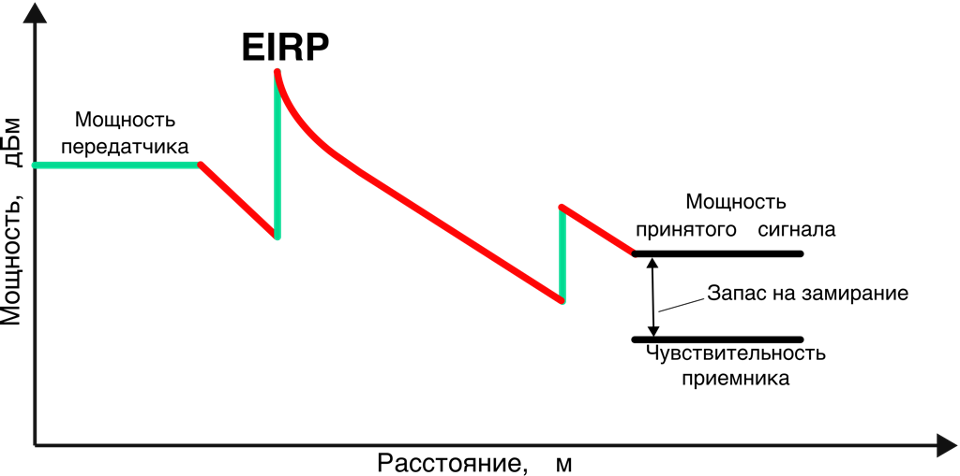
\includegraphics[width=1\textwidth]{link_power.png}
\caption{Энергетический потенциал линии связи.}
\label{fig:link_power}
\end{figure}

На стороне передатчика выходной мощностью является величина, равная мощности, подводимой к антенне. Данная величина из паспортной документации устройства имеет различные значения в зависимости от каждого поддерживаемого оборудованием стандарта и конкретных скоростей. В реальной условиях значения мощностей, как правило могут незначительно отклоняться от паспортных значений. Предельная мощность передатчика определяется государственными органами. Для примера, для БШС семейства протоколов IEEE 802.11 не превышает 100 мВт или, выражая в децибеллах, не боллее 20 дБм \cite{GKRCh18_13}.


Затухание сигнала могут происходить в кабелях антенны, зависящие от типа кабеля и рабочей частоты. При подключении антенны желательно обходиться минимальной длиной кабеля. Потери сигнала в антенном кабеле принимают $0, 1...2$ дБ/м. В технической документации в потерях кабеля также учтена величина затухания в кабельных разъемах. 

Усиление антенны описывает фокусирование переданного или полученного сигнала. Значения даны относительно полуволнового диполя или теоретического изотропного излучателя \cite{Gost62657}.


К потерям при распространении относятся все виды затухания сигнала, которые имеют место при его распространении от антенны передатчика к антенне приемника. Самая простая оценка потерь в свободном пространстве получается, если предположить, что сигналы передаются во всех направлениях, то есть мощность излучается одинаково во всех направлениях, и в зоне передачи или вокруг нее нет препятствий, которые могли бы повлиять на распространение электромагнитных сигналов \cite{Krouk2010}. 

% Передающий сигнал рассеивается по мере увеличиня расстояния между приемником и передатчиком. Данный тип затухания называется потерями в свободном пространстве (Free Space Path Loss, $FSPL$).

\subsection{Модель потерь в свободном пространстве}
При распространении сигнала от передатчика к приемнику часть сигнала рассеивается, по этой причине мощность на приемной стороне будет уменьшаться с увеличением  расстоянии от передающей антенны. Данное затухание сигнала называют потерями в свободном пространстве (Free Space Path Loss, $FSPL$).

Потери при распространении между двумя неизотропными антеннами в свободном пространстве (в воздухе) можно выразить из уравнения Фрииса \cref{eq:part1_Friis}:

% \begin{equation}
%   \label{eq:part3_FSPL}
%   FSPL = \left(\frac{4\pi R f}{c} \right)^2.
% \end{equation}

% Формула \cref{eq:part3_FSPL}, выраженная в децибеллах будет выражаться как

Мощность принимаемой антенны рассчитывается из уравнения передачи Фрииса:

\begin{equation}
  \label{eq:part1_Friis}
  \frac{P_{recv}}{P_{tr}} = G_{tr}G_{recv}\left(\frac{c}{4\pi R f} \right)^2,
\end{equation}
где
$c$ --  скорость света,
$f$ -- частота, 
$R$ расстояние между приемной и передающей антенной.

\begin{equation}
  \label{eq:part3_L_fs}
  L_{fs} = 20 \lg{F} + 20\lg{R} - G_{tr} - G_{recv} + K,
  \end{equation}
где $F$ -- центральная частота, на котором работает канал связи, $R$ -- расстояние между приемной и передающей антенной и $K$ -- константа.

Константа $K$ зависит от размерностей частоты и расстояния:

\begin{itemize}
  \item для частоты, выраженной в ГГц, и расстояния, выраженная в км, константа $K$ равна 92.45;
  \item для частоты, выраженной в МГц, и расстояния, выраженная в км, константа $K$ равна 32.4;
  \item для частоты, выраженной в МГц, и расстояния, выраженная в м, константа $K$ равна -27.55.
\end{itemize} 

Потери $L_{fs}$ выразим из уравнения энергетического потенциала канала связи \cref{eq:part3_link_budget} как:

\begin{equation}
  \label{eq:part3_L_fs_from_link_budget}
  L_{fs} = P_{tr} - L_{tr} + G_{tr} + G_{recv} - L_{recv} - SOM - P_{recv}.
\end{equation}


Запас на замирание сигнала, SOM,  учитывает все возможные факторы отрицательно влияющие на дальность связи. К таким факторам относятся:

\begin{itemize}
  \item температурный дрейф чувствительности приемника и выходной мощности передатчика;
  \item влияние погодных условий на передачу сигнала: туман, снег, дождь;
  \item  потери в антенно-фидерном тракте, возникающие из-за рассогласования фидера и антенны.
\end{itemize}
Приемник испытывает совокупное воздействие всех этих физических факторов, которые различаются в зависимости от положения приемника и передатчика в среде распространения. 

Минимальная значения величины запаса на замирание  (System Operating Margin, $SOM$) должна быть не меньше  10 дБ. Считается, что 10-ти децибельный запас по усилению достаточен для инженерного расчета, но на практике зачастую используют значение $20 ... 30$ дБ \cite{Proletarsky}.

% \fixme{Энергетический потенциал указывает на качество канала передачи радиосигналов}.



% The Free Space Path Loss ($ FSPL $) equation defines the propagation signal loss between two antennas through free space (air):



Максимально возможную дальность связи между приемником и передатчиком выводится из уравнений \cref{eq:part3_L_fs} и \cref{eq:part3_L_fs_from_link_budget}:

\begin{equation}
  \label{eq:part3_D}
  R = 10^\frac{L_{fs} - 20\lg{F} + G_{tr} + G_{recv} - K}{20}.
\end{equation}

Используя формулу \cref{eq:part3_D} и \cref{eq:part3_L_fs_from_link_budget}, мы можем расчитать теоретическое максимальную дальность связи $ R_{jq}$ между базовыми станциями и радиусом покрытия $ r_j $ с предположением об отсутствии препятствий, отражений, влияния контуров местности и т. д. Это допущение приемлемо для нашего случая с открытой местностью.

\begin{figure}[h!]
  \centering
   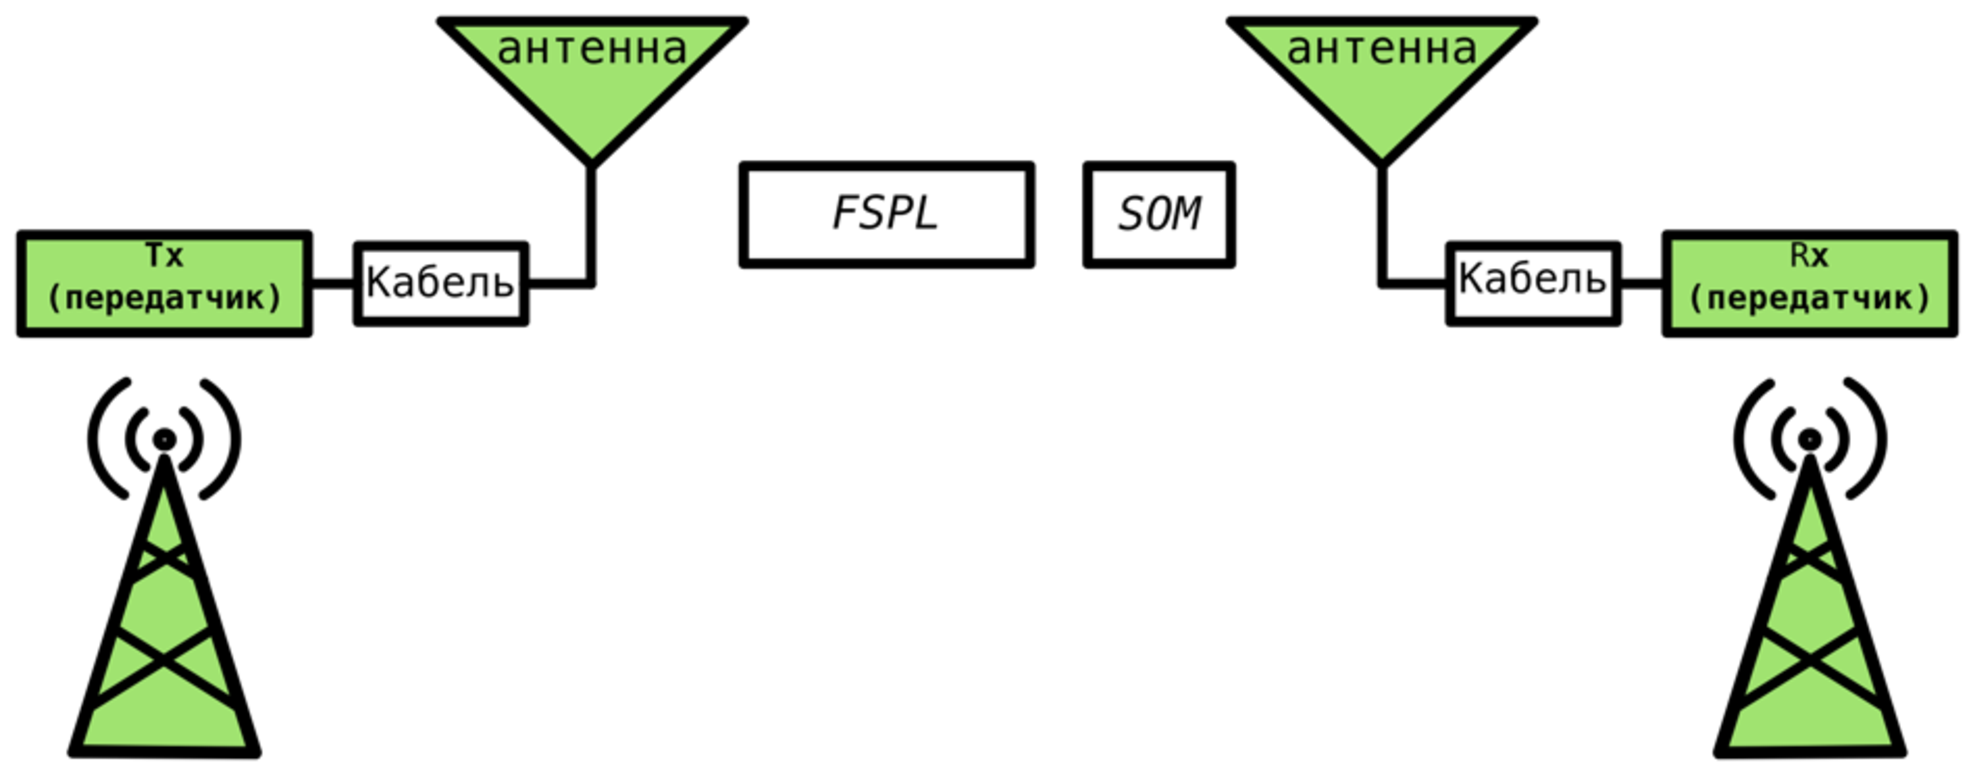
\includegraphics[width=0.8\textwidth]{link_distance.pdf}
\caption{Соединение между станциями.}
\label{fig:part3_link_distance}
\end{figure}

Для расчета дальности связи $R_{jq}$ (Рисунок \cref{fig:part3_link_distance}), базовые станции $s_j$ и $s_q$ будут рассматриваться как станции \textit{передатчик} и \textit{приемник}, соответственно. Будем считать, что станции оборудованы направленными антеннами с усилениями $G_{tr}^{R}$ и $G_{recv}^{R}$.

\begin{figure}[h!]
  \centering
   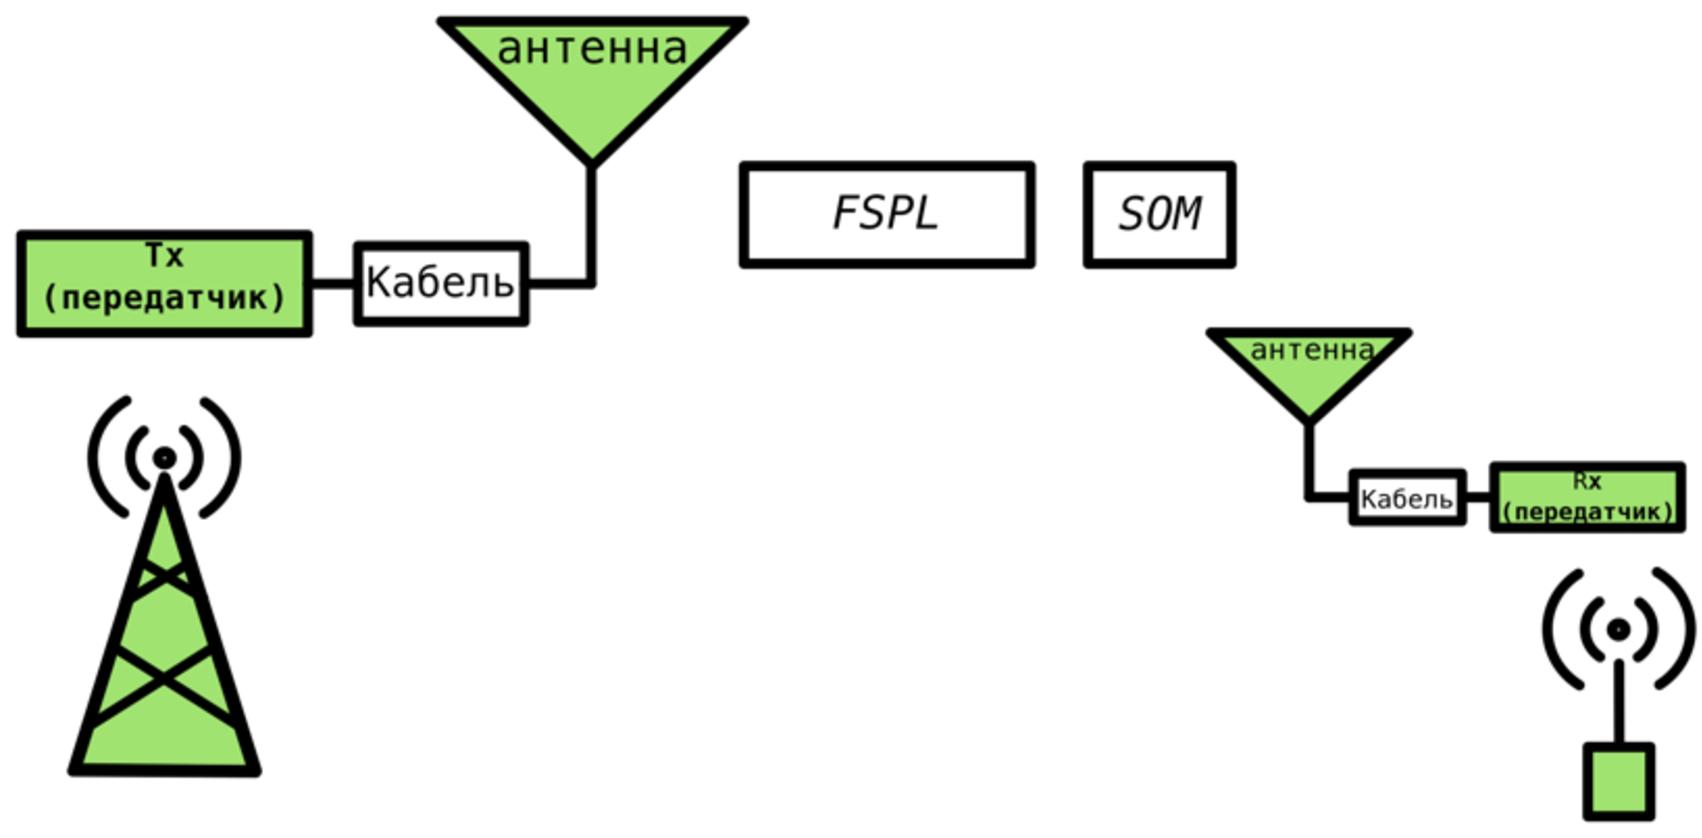
\includegraphics[width=0.8\textwidth]{coverage.pdf}
\caption{Покрытие станции}
\label{fig:part3_coverage}
\end{figure}

Каждая базовая станция оснащена всенаправленной антенной с заданным усилением антенны $G_ {tr}^{r}$. Данная антенн необходимо для покрытия заданной области.

% Each base station is equipped with an omnidirectional antenna with given gain antenna $G_{tr}^{r}$. A station uses this antenna to cover a given area.

При вычислении радиуса покрытия $r_j$ (Рисунок  \cref{fig:part3_coverage}) базовая станция будем считать \textit{передатчиком}, а пользовательское устройство \textit{приемником}.

\subsection{Модель распространения SUI}

Модель распространения SUI (Stanford University Intern) предложена рабочей группой, занимающаяся исследованием беспроводной широкополосной сети IEEE 802.16 \cite{Mollel2014}. Модель включена в стандарты IEEE и широко используется в WiMax, а также в LTE \cite{Zreikat2017}. Подходит для использования в сельской местности с различным типом рельефа, а также в небольших населенных пунктах. Модель испытана на равнинах, пересеченной, холмистой местности и лесных массивах. SUI модель используется для диапазона частот 1900 МГц -- 11 Ггц \cite{Cabuk2020}. Высоты антенн БС в диапазоне от 10 до 80 м, высота антенны мобильного устройства –- от 2 до 10 м, расстояние между БС и устройством от 0,1 до 8 км.

Грубая оценка потери сигнал описывается с помощью модели SUI как

\begin{equation}
  \label{eq:part1_sui_l0}
  L_0 = A + 10\gamma\lg{(R/R_0)},
\end{equation}
$$
A = 20\lg{(\frac{4\pi R_0 }{\lambda})}
$$
и
$$
\gamma = a - b h_t + \frac{c}{h_t}, 
$$
где $R$ -- дальность связи, $R_0$ -- минимальная разрешенная дальность (100 м), $\lambda = c / f$ -- длина волны, $f$ -- частота в МГц, $h_t$ -- высота антенны БС, $h_r$ -- высоты антенны устройства. Параметры $a, b$ и $c$, определяющие следующие типы местности (Таблица \cref{tab:part1_abc_sui_model}):
\begin{itemize}
  \item тип A -- холмистая местность или густые лесные массивы;
  \item тип B -- пересеченная местность или полугустые лесные массивы;
  \item тип C -- открытые поля.
\end{itemize}


\begin{longtable}[c]{| c | c | c | c |}
  \caption{Численные значения параметров модели SUI.}\label{tab:part1_abc_sui_model}\\

  \hline
  \textbf{Параметры модели} & \textbf{Местность A} & \textbf{Местность B} &  \textbf{Местность C}\\ \hline
  a & 4,6 & 4 & 3.6 \\
  b & 0,0075 & 0,0065 & 0.005 \\
  c & 12,6 & 17,1 &20 \\
  \hline
  \hline
\end{longtable}




\fixme{ДОДЕЛАТЬ SUI И ДОБАВИТЬ ДВУХЛУЧЕВУЮ}

Формула \cref{eq:part1_sui_l0} была получена эмпирически для несущей частоты 2 ГГц и высоты приемника 2 м. Для использования модели с другими частотами и высотами необходимо добавить поправочные коэффициенты 

\begin{equation}
  \label{eq:part1_sui_lfs}
  L_{fs} = L_0 + \Delta L_f + \Delta L_h + s,
\end{equation}
где $\Delta L_f$ -- корректирующий коэффициент для частот свыше 2 ГГц $\Delta L_h$ --  корректирующий фактор высоты антенны устройства (м) $s$ -- корректирующий фактор теневого эффекта, имеющий значения в диапазоне $8,2 < S < 10,6$ дБ. Параметр $\Delta L_f$ рассчитывается 
$$
\Delta L_f  = 6 \lg{(f / 2000)},
$$
параметр $\Delta L_h$ выбирается исходя из выбора типа местности

$$
\Delta L_h =  
 \begin{cases}
  -10,8 \lg{(h_r/2)} &\text{для типа A и B,}\\
  -20 \lg{(h_r/2)} &\text{для типа C.}
 \end{cases}
$$

Из уравнений \cref{eq:part1_sui_l0, eq:part1_sui_lfs} можно вывести дальность действия связи:

\begin{equation}
  R = 10^{(\frac{L_{fs} - L_0 - \Delta L_f - \Delta L_h - s - A}{10\gamma} + \lg{R_0})}
\end{equation}

\subsection{Модель двух лучевого распространения}

Двух лучевая модель описывает мощность принятого сигнала как интерференцию двух копий переданного сигнала: первая -- луч прямой видимости, вторая -- отраженная от поверхности \cite{Gaitan2020}. 
Два луча электромагнитных волн от передатчика приходят в приемник с определенной разностью фаз и амплитуд. Разность фаз происходит из-за дополнительного времени распространения волны, отраженного от земли \cite{Rademacher2016, Bacco2014, Zochmann2017, Kurt2017}. 

\fixme{Проверить}

Мощность принимаемого сигнала, в соответствии с двухлучевой моделью равна

\begin{equation}
  \label{eq:part1_two-ray_model_prcev}
  P_{recv} = \frac{P_{tr} \cdot G_{tr} \cdot G_{recv} \cdot h^2_{tr} \cdot h^2_{recv}}{R^4},
\end{equation}
где $P_{recv}$ -- чувствительность приемника, $P_{tr}$ -- мощность передатчика,$G_{tr}$ -- усиление антенны передатчика, $G_{recv}$ -- усиление антенны приемника, $h_{tr}$ -- высота передатчика, $h_{recv}$ -- высота приемника, $R$ -- расстояние между приемником и передатчиком.

Потери в свободном пространстве из формулы \cref{eq:part1_two-ray_model_prcev} вычисляются как:

\begin{equation}
  \label{eq:part1_two-ray_model_lfs}
  L_{fs} = 40\lg{R} - 10\lg{G_{tr}} - 10\lg{G_{recv}} - 20\lg{h_{tr}} - 20\lg{h_{recv}},
\end{equation}

Тогда из формулы \cref{eq:part1_two-ray_model_lfs} дальность рассчитывается как

\begin{equation}
  \label{eq:part1_two-ray_model_r}
  R = 10^\frac{L_{fs} + 10\lg{G_{tr}} + 10\lg{G_{recv}} + 20\lg{h_{tr}h_{recv}}}{40}.
\end{equation}

\fixme{ПЕРЕДЕЛАТЬ ФОРМУЛУ ФРИИСА, ЧТОБЫ УЧИТЫВАТЬ НЕИЗОТРОПНЫЕ АНТЕННЫ}

\fixme{ВЕЗДЕ ПРОВЕРИТЬ ЛОГАРИФМ ПО ОСНОВАНИЮ 10}

\subsection{\fixme{Расчет параметров БС, необходимых для задач оптимизации}}

\section{Оценка характеристик производительности сети с помощью стохастических моделей массового обслуживания}

\subsection{\fixme{Время передачи пакета в канале}}

\begin{itemize}
  \item Структура кадра;
  \item Время передачи 
\end{itemize}

Стандарт IEEE 802.11 описывает три типа кадров \cite{Proletarsky}:
\begin{itemize}
  \item кадры данных -- используются для передачи данных передачи данных;
  \item контрольные кадры -- служат для управления доступом к среде передачи данных;
  \item кадры управления -- используются для обмена управляющей информацией при выполнении таких операций подуровня MAC.
\end{itemize}

\fixme{RTS/ CTS станции ждут NAV}

\fixme{В 802.11e добавили AIFS}

\fixme{Окно конкуренции.} Выбирается псевдослучайное число равномерного распределения в интервале $[0, CW]$

\fixme{EIFS -- если кадр пришел с ошибкой}

\fixme{Время передачи пакета в канале - это время как станция впервые решила передавать кадр до момента получения ACK об успешной доставке}


Основой стандарта 802.11 является распределенная функция координация DCF. Согласно данному механизму, станция, желающая передать пакет данных, слушает шумы в передающей среде в течение заранее определённого периода времени. Если передающая среда свободна, станция может передавать пакеты. В противном случае станция должна ждать определённое количество времени, прежде чем опять предпринять попытку отправки пакета.

Процедура Backoff (Рисунок \cref{fig:part1_interframe_time}).

\begin{figure}[h!]
  \centering
   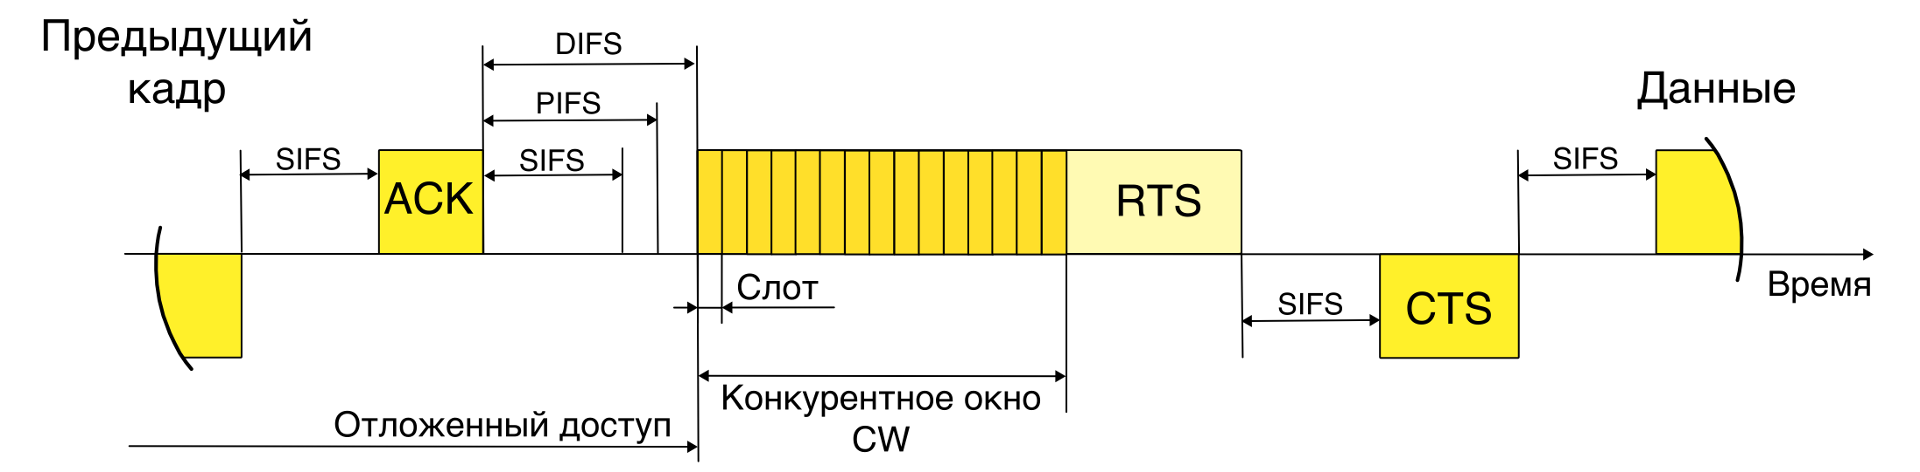
\includegraphics[width=1\textwidth]{interframe_time.png}
\caption{Процедура Backoff}
\label{fig:part1_interframe_time}
\end{figure}
 
  
\textbf{Борьба с коллизией}

В соответствии c алгоритмом RTS/CTS каждый узел сети, перед тем как послать данные в «эфир», сначала отправляет специальное короткое сообщение, которое называется RTS (Ready To Send) и означает готовность данного узла к отправке данных. Такое RTS-сообщение содержит информацию о продолжительности предстоящей передачи и об адресате и доступно всем узлам в сети (если только они не скрыты от отправителя). Это позволяет другим узлам задержать передачу на время, равное объявленной длительности сообщения. Приемная станция, получив сигнал RTS, отвечает посылкой сигнала CTS (Clear To Send), свидетельствующего о готовности станции к приему информации. После этого передающая станция посылает пакет данных, а приемная станция должна передать кадр ACK, подтверждающий безошибочный прием. 

 
CSMA/CA 

Станция дожидается бездействие канала в течение короткого периода времени \textbf{DIFS} и отсчитывает слоты бездействия, приостанавливает отсчет на время отправки кадров. Свой кадр она отправляет, когда счетчик достигает нуля. Если кадр передался успешно, на приемник отправляет передатчику короткое подтверждение. Если подтверждение нет, передатчик делает вывод об ошибке \cite{Tanenbaum2022}. В таком случае отправитель удваивает период молчания и повторяет передачи кадра, продолжая экспоненциально увеличивать длину паузы. Увеличение длины происходит, пока кадр успешно не будет передан или не будет достигнуто максимальное число повторов.


Каждый кадр содержит поле \textbf{NAV} (Network Allocation Vector) -- вектор распределения сети, которое сообщает, как долго последовательность кадров будет передаваться. Все станции, услышавшие этот кадр, понимает, что канал занят в течение периода времени \textbf{NAV}.

Самый короткий интервал времени --  короткий межкадровый интервал (Short InterFrame Interval, \textbf{SIFS}). Интервал SIFS используется для того, чтобы одна из станций могла начать первой. 

Для того чтобы обеспечить приоритизацию передачи трафика в 802.11е добавили механизм обеспечения качества обслуживания. Существует межкадровый арбитражный интервал (Arbitration InterFrame Space, \textbf{AIFS}).

\subsection{Расчет межконцевой задержки}\label{part4_e2e_delay_section}

Как уже было отмечено ранее, одним из важных ключевых задач при проектировании БШС является оценка ее характеристик производительности для удовлетворения требуемого качества обслуживания (quality of service, QoS). Одной из основных характеристик проектируемой сети является ее межконцевая задержка \cite{Vishnevsky2016_Methods_of_performance, Wang2017, Liu2016, Chen2019, Hosni2017, Capone2019, Abbas2017, Seliem2019, Malandra2018, Kalor2018, Larionov2019, Gao2016}. Для расчета сквозной задержки сети используют стохастические модели массового обслуживания \cite{Vishnevsky2016_Methods_of_performance, Wang2017, Liu2016, Malandra2018, Larionov2019, Gao2016}. 

Пусть задан частной случай БШС. Все БС связаны последовательно между собой в сеть с линейной топологией. Для расчета межконцевой задержки в простейшем случае рассмотрим беспроводную сеть как сеть массового обслуживания (СеМО) с кросс-трафиком и узлами $M/M/1$ (Рисунок \cref{fig:tandem_queue}). 

Узлами сети являются БС. Согласно символике Дж. Кендала, обозначение $M$ указывает на показательное распределение случайной величины \cite{VishnevskyBook, Kleinrock1975}. Каждая такая БC характеризуется случайными величинами входящего потоком пакетов и временем их обслуживания, принадлежащие экспоненциальному закону распределения. Каждый узел имеет один обслуживающий прибор. Для такой СеМО принято допущение о бесконечном размере буфера, в котором пакеты ожидают своего обслуживания. Данное допущение позволяет получить аналитическое решение, которое возможно использовать для проивзольного размера СеМО для данной топологии.

\begin{figure}[h!]
  \centering
   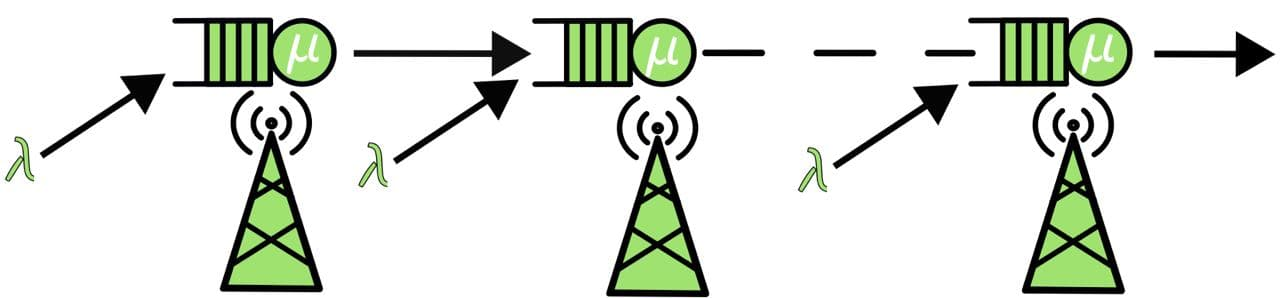
\includegraphics[width=1\textwidth]{tandem_queue.png}
\caption{СеМО с кросс-трафиком и узлами $M/M/1$}
\label{fig:tandem_queue}
\end{figure}

На вход каждой станции поступает пуассоновский поток. Пуассоновский процесс представляет собой случайный процесс, характеризующийся  экспоненциально распределенным временем между событиями. Это один из наиболее важных случайных процессов в теории вероятностей, который широко используется для моделирования поведения трафика и входов во многих коммуникационных сетях и системах \cite{Kalor2018, Gao2016, Malandra2018, Seliem2019}. 

В пуассоновском процессе события происходят непрерывно и независимо друг от друга. Функция распределения имеет вид  \cite{VishnevskyBook, Kleinrock1975}:

\begin{displaymath}
P(X<x) = 
  \begin{cases}
    1 - e^{- \lambda x}, \quad x \geqslant 0; \\
    0, \quad x < 0.\\
  \end{cases}
\end{displaymath}

Для входящего потока, интервалы между поступлениями заданны случайной величиной c экспоненциальным распределением и интенсивностью $\lambda$. Время обслуживания на узле задана также экспоненциальным распределением и интенсивностью $\mu$. 


По теореме Бурке \cite{Burke1956}, поток на выходе узла $M/M/1$, а значит на входе каждой последующей фазы тоже пуассоновский. Интенсивность на выходе каждой фазы равна суммарной интенсивности всех входящих потоков с интенсивностями $\lambda$.

Пропускная способность на практике часто составляет половину от заданной в спецификации оборудования \cite{Proletarsky, Vladimirov2019}. Интенсивность времени обслуживания рассчитывается по формуле: 

\begin{displaymath}
    \mu_j = 0.5 \cdot p_j / w,
\end{displaymath}
где: $p_j$ - пропускная способность $j$-ой станции, Мбит/с; $w$ - средний размер пакета, Мбит.

Для каждой станции коэффициент загрузки равен:


\begin{displaymath}
\rho_j= \frac{\sum{\lambda}}{\mu_j} = \frac{q \cdot \lambda}{\mu_j} <1,
\end{displaymath}
где $q$ -- число входящих потоков. Условие $\rho_j<1$ является необходимым и достаточным условием существования стационарного режима функционирования СеМО.

Далее по формуле Литтла \cite{Little1961} можно рассчитать время задержки на каждой станции:

\begin{displaymath}
    \overline{T_j} = \frac{\rho_j}{1 - \rho_j} \cdot \frac{1}{q \cdot \lambda}.
\end{displaymath}

Тогда межконцевая задержки в сети равна

\begin{equation}
    \label{eq:end_to_end_delay}
    \overline{T}= \sum{\overline{T_j}}.
\end{equation}


Существуют более сложные модели очередей для оценок характеристик с более сложными распределения входящего трафика и времени обслуживания. Адекватные оценки дают модели с коррелированными входным потоком \cite{Vishnevsky2016_Methods_of_performance, Larionov2019}. К сожалению, такие модели труднорешаемы и для большего числа фаз СеМО не имеют аналитических расчетов. В данном исследовании будем использовать простейшую модель СеМО с узлами $M/M/1$ на этапе задачи оптимального размещения. Согласно предложенной концепции проектирования, полученную БШС с размещенными БС и выбранным техническим оборудованием можно будет в дальнейшем проводить на более сложных моделей на следующем этапе моделирования сети. Этот этап включает в себя математическое, имитационное моделирования для оценок характеристик производительности как время задержек, длины очередей, пропускная способность, вероятность потери пакетов и др. Данный этап позволяет провести комплексную проверку соответствия QoS для полученного размещения БС.

\section{Выводы по главе 1}
 
В главе представлено актуальность внедрения БШС в рамках цифровой трансформации нефтегазового сектора <<Индустрия 4.0>>. Представлены тематика исследования и задачи, затронутые в диссертации в рамках данного внедрения, а именно задачи синтеза топологии при проектировании беспроводных телекоммуникации на месторождении. Представлена структура последовательностей этапов при проектировании и место задачи синтеза в ней. Представлены методика расчета 
параметров БС необходимых в дальнейшем для оптимизационных задач размещения БС. 



% \begin{figure}[h!]
%   \centering
%    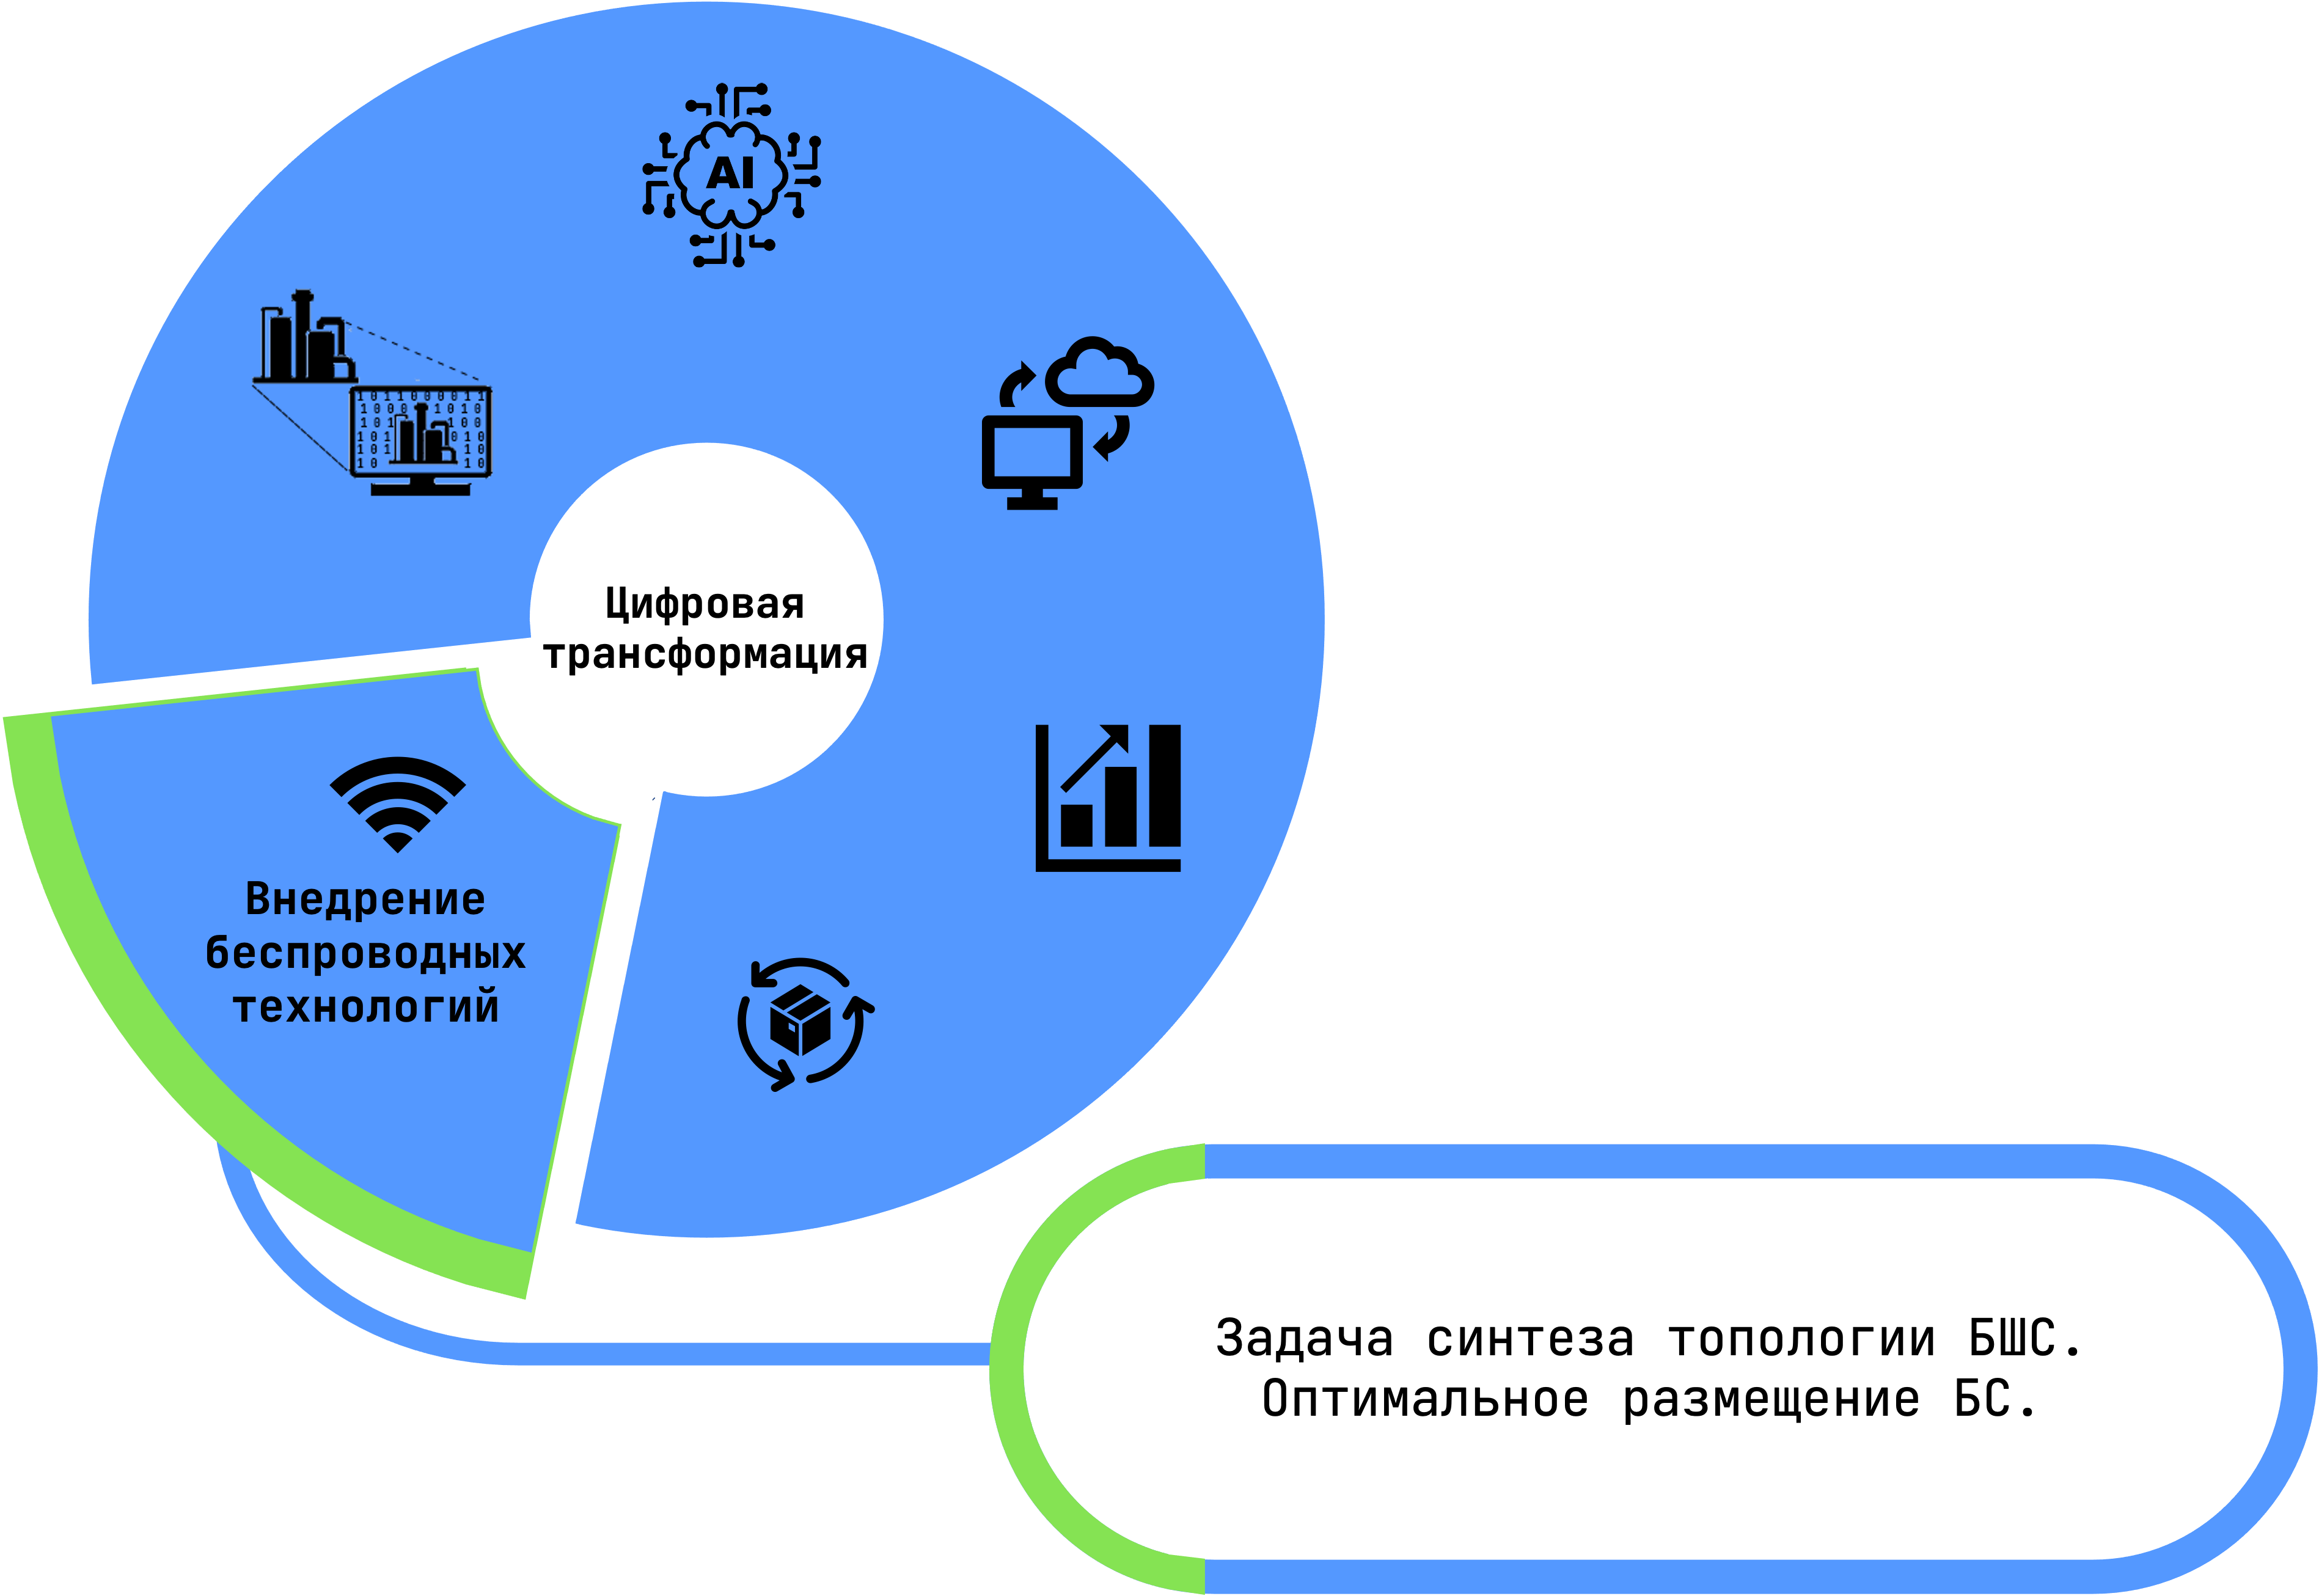
\includegraphics[width=1\textwidth]{industry4.png}
% \caption{Задача синтеза топологии при проектировании БШС в рамках цифровой трансформации "Индустрия 4.0".}
% \label{fig:industry4}
% \end{figure}





\FloatBarrier
